\documentclass[12pt,a4paper,titlepage = false,twoside, bibliography=totoc]{scrreprt}

\usepackage[bottom=3cm, top=2.5cm, left=2cm, right=2cm, bindingoffset=10mm]{geometry}                % specify geometry of the pages

%% Packages
%% ------------------------------------------------------------------
\usepackage{typearea}
\usepackage[utf8]{inputenc}
\usepackage[T1]{fontenc}
\usepackage[english]{babel}
%\usepackage{floatpag}              % Different pagestyles
\usepackage{amsmath}
\usepackage{mathtools}
\usepackage{booktabs}               % Is needed for \toprule f.e. in tables
\usepackage{array}                  % Extending the array and tabular environments
\usepackage{setspace}               % Set space between lines (\onehalfspacing, \doublespacing)
%\usepackage{cancel}                 % Strike out things with \cancel{tostrikeout}
\usepackage[usenames,dvipsnames]{xcolor}

\usepackage{amsfonts}
%\usepackage[cc]{titlepic}          % Enables ONE picture on titlepage
\usepackage{amssymb}
\usepackage{graphicx}
\usepackage{tabularx}
\usepackage{epstopdf}
\usepackage{pifont}
\usepackage{natbib}
%\usepackage{cite}
\usepackage[automark]{scrpage2}
\usepackage{float}
\usepackage{caption}
\usepackage{subcaption}
\captionsetup[sub]{justification=centering}
%\usepackage{makeplot}
\usepackage[toc,page]{appendix}     % for making an appendix
\usepackage[hyphens]{url}           % prints URLs like they should be in bibtex
\usepackage{wrapfig}                % Floating figures
\usepackage{abstract}               % adds the word "Abstract" and modifications can be made
%\usepackage{bibtopic}               % Several bibtex files within one document
% \usepackage[labelfont={color=brown,bf},font={small},singlelinecheck=false,format=plain,justification=justified,indention=0cm]{caption}
\usepackage{hyperref}               % Makes active (on click) references in the final pdf
\usepackage{afterpage}              % Execute command after the next page break
\usepackage{placeins}               % Control float placement with /FloatBarrier


\usepackage{upgreek}
%\usepackage{sistyle}                   % Package to typeset SI units
%\usepackage{titlesec}

%% New Commands
%% ----------------------------------------------------------------------------------

\newcommand{\chapterauthor}{}
\newcommand{\nn}{\ensuremath{\mathrel{\nonumber}}}


%\titleformat{\chapter}                  % command to format the chapter titles
%        [hang]                          % shape/type of title
%        {\LARGE\bfseries}
%        {\makebox[0.5in][l]{\thechapter}}
%        {0em}
%        {}
%        [
%            \normalsize\normalfont      % reset font formatting
%            \vspace{0.5\baselineskip}
%            \hspace*{0.5in}             % indent author name width of chapter number box
%            \large                      % make text that follows large
%            \thispagestyle{empty}       % suppress page numbers
%            \textit{\chapterauthor}
%        ]                               % end of what comes after title


%\titlespacing*{\chapter}
%     {0em}                              % spacing to left of chapter title
%     {0ex}                              % vertical space before title
%     {3\baselineskip}                   % vertical spacing after title; here set to 3 lines 


\newcommand{\todo}[1]{\textbf{\textcolor{red}{#1}}}
\newcommand{\degc}{$^\circ$C}
\newcommand{\edegc}{^\circ \text{C}}


%% Miscellaneous Settings
%% --------------------------------------------------------------------------

% \setlength{\parindent}{0mm}

\setheadsepline{1pt}

\pagestyle{scrheadings}



%% Main Document Part
%% -------------------------------------------------------------------------------

%%%%%%%%%%%%%%%%%%% Title %%%%%%%%%%%%%%%%%%%%%%%%%%

\title{Here could be your title}
\author{A. Uthor}
\date{\today}

%%%%%%%%%%%%%%%%% Document %%%%%%%%%%%%%%%%%%%%%%%%%%%

\begin{document}

%\maketitle

\setcounter{tocdepth}{2}
\tableofcontents
\bibliographystyle{AGFstyle}

\clearpage

%%%%%%%%%%%%%%%%% PREFACE %%%%%%%%%%%%%%%%%
%\chapter*{Preface}
%\addcontentsline{toc}{chapter}{Preface}
%Fieldwork is an important part in most courses at UNIS...

%%%%%%%%%%%%%%%% SINGLE REPORTS %%%%%%%%%%%

% Each student should work in such a file! In that case you have to add all this documents text into the MainPart.tex file to compile it. Each student should work with this header and shouldn't add any packages, otherwise it might not work in the end by connecting all parts.
% The header has to be deleted in all ReportPart.tex files, before connecting!

%%%%%%%%%%%%%%%%%%%%% Write your name here!! %%%%%%%%%%%%%%%%%%%%%

\renewcommand{\chapterauthor}{Moritz Bitterling, Linda Thielke, Julien-Pooya Weihs}
\chapter{Ice velocity measured by differential GPS}
\label{gpsmeas}

%--------------- Abstract ----------------------
\begin{abstract}
The aim of this report is to measure the ice velocity on the glaciers of Tellbreen and Blekumbreen (Adventdalen, Svalbard) with the differential Global Positioning System (dGPS) method. This method with a higher accuracy than the Global Positioning System (GPS) was necessary to address behaviours of very small velocities.
A new open-source post-processing method is applied and suggestions of long-term and convincing replacement of the former method are provided to slowly transition away from the restricted Trimble Business Center post-processing work-flow.
The average uncertainties of our calculated velocities are 0.40 [m] for Northing, 0.19 [m] for Easting, 0.89 [m] for the elevation, and are as such are larger than the calculated velocities themselves, making it impossible to determine an ice velocity for any stake on either of the two glaciers. This conclusion induces an irrelevancy to perform further calculation on the ice fluxes and their directions.
The mass balance of the glacier is calculated through the change of elevation in time at each stake. 
The mass balance gradient is of 5.1 $\pm$ 1.0 [mm/m] on Tellbreen and of 6.8 $\pm$ 1.4 [mm/m] on Blekumbreen. The altitudes of the theoretical equilibrium lines at 757 $\pm$ 56 [m] for Tellbreen and 751 $\pm$ 45 [m] for Blekumbreen are higher than the highest point of any of the two glaciers. Both glaciers are situated in their own ablation zone.
We verify our measurements with the theoretical model of the \textit{shallow ice} approximation. The theoretical velocity values have orders of magnitude of centimeters per year for reasonable assumptions of slope angles, ice viscosities and ice thicknesses. Their results confirm our measurement results with a slow movement of both glaciers.
\end{abstract}
%-----------------------------------------------

%-------------- Chapters -------------------

\section{Introduction}
Many topics in glaciology call for an understanding of the velocity field in a glacier. 
In fact, the way in which the flow redistributes mass is directly connected to a glacier's shape. But flow also induces energy redistribution and as such, the temperature distribution, which itself has implications for the nature of the coupling with the glacier bed. 
Spatial variations in speed, also known as strain rates $\epsilon$, are being studied by structural geologists who use glaciers as analogs for rock deformation. 
From a geomorphic point of view as well, the entrainment of debris and the different moraines they construct depend upon the flow field too. 
Understanding those velocity fields therefore is fundamental to the analysis of a number of problems in glacier mechanics.
We used the differential Global Positioning Sytem (dGPS) to get accurate data on the mass balance stakes' postions.
We rely on these measurements to extract experimental values for the surface velocity of the glacier, comparing previous positions from the last years to the new ones.
We also address the data treatement algorithm as we strive for a clear understanding of the processing.
In that scope we introduce, with the open source post processing, a new method that allows a transparent step by step understanding of the work flow.
For consistency howerver we also conducted the Trimble Business Center post processing to asure continuity with the previous years' results. 
We focused on the measurement method because the results from the last years were unclear and could not provide a real movement of the glacier.
We therefore thought important to emphasize on the analysis of the measurement methods and their uncertainties, and herewith suggest a more rigourous protocol aiming at a more durable and reliable data collection on the field.
\medskip 

The chapter on theory walks us through the calculation of the horizontal velocity in a glacier. After having motivated the computation of the surface velocity through the \textit{shallow ice approximation}, we relate it to a depth-averaged velocity. Using this result, we make an assumption on the glacier's cross-section around each stake we probed and present a value for the ice flux of each glacier's delimited part. Finally, we cross-check our results with those of the mass-balance group and draw a conclusion relating to the \textit{steady state assumption}.
In the processing part the final position determined by the post processing with base station data and the stake correction caused by uncertainties in our setup in the field.
Based on this, it is important to consider the propagation of uncertainties.
With the position data, including northing, easting and elevation, the velocity of every stake can be calculated by the differnce of the stake positions of the last years.
Next to the horizontal velocity, it was possible to calculate the vertical velocity to determine a mass balance for our measurement sites. 
Finally, the discussion and conclusion close the report.


\section{Theoretical background} \label{GPS:sec:Theoretical backround}
%\usepackage[parfill]{parskip}   
%
%\usepackage{bm}

%\section{}
%\subsection{}
%\chapter{}

%\begin{equation}...\end{equation}

%\begin{center}
%\end{center}

%\begin{itemize}
%\item blah blah
%\end{itemize}

%\begin{description}
%\item blah blah
%\end{description}

%\begin{enumerate}
%\item blah blah
%\end{enumerate}

%\begin{flushright}
%\end{flushright}

%\begin{figure}
%	\begin{center}
%		\includegraphics[scale=0.7]{nomdupdf}
%		\caption{Graphique}
%	\end{center}
%\end{figure}

%\listoffigures
%\listoftables

%\label{etiquette}
%\ref{etiquette}
%\pageref{etiquette}

%\begin{align*}
%A&=B\\
%&=C\\
%&=D
%\end{align*}

%\fbox


%\newcommand{\fraction}[2]{\raisebox{0.5ex}{#1} \slash \raisebox{-0.5ex}{#2}}


\subsection*{Ice velocities using the stake positions of the previous year}

If we define each measured position of the mass balance stakes by $P_i(x,y,z)$ where $P$ accounts for the codename of the stake and $i$ labels the year of the considered stake, the horizontal distance $d$ between a stake $P_a(x_a, y_a, z_a)$ and $P_b(x_b, y_b, z_b)$ is given by :

\begin{equation}d = \sqrt{(x_a - x_b)^2 + (y_a - y_b)^2}\end{equation}

The horizontal surface velocity $u_s$ is calculated through :

\begin{equation}
\boxed{u_s = \frac{d}{t_{a \rightarrow b}}}
\end{equation}

where $t_{a \rightarrow b}$ is the elapsed time between the measurements $a$ and $b$.


\subsection*{Relating the surface velocity to depth-averaged ice velocity}

Now that we have the horizontal surface velocity, we wonder how it evolves with depth. Nye \cite{Nye1952} has proven that the overlying ice of a glacier must move at least as fast as that below. In quantitative terms, this translates to a reasoning that starts with the flow law for the strain rate $\dot{\epsilon}$ :

\begin{equation}\dot{\epsilon} = \left( \frac{\sigma}{B} \right)^n\end{equation}

with $\sigma$ a dominant shear stress, $B$ an ice viscosity parameter that is temperature dependent and increases with the stiffness of the ice, and $n$ the constant creep exponent. The latter has often experimentally proven to be $n \approx 3$, but for the sake of the derivation, we'll keep the value variable.
This law is also named after Glen's \cite{Glen1955}, who conducted the first uniaxial compression experiments on ice.

We will follow up with the assumptions of the layer we consider being parallel-sided, that there's no flow in $y$ direction and that everything is uniform in $x$, $y$, as depicted in the \textsc{Figure} \ref{velocities}. The stress rate tensor therefore comes down to :


\begin{equation} \dot{\epsilon} = \left( \begin{array}{ccc}
0 & 0 & \dot{\epsilon}_{xz} \\
0 & 0 & 0 \\
\dot{\epsilon}_{zx} & 0 & 0
\end{array} \right) \end{equation}

From the constitutive relations, linking the stress $\sigma$ to the strain $\epsilon$ component per component, it follows that $\sigma_{xz} = \sigma_{zx}$ and hence :

\begin{equation}\dot{\epsilon}_{zx} = \left( \frac{\sigma_{zx}}{B} \right)^n\end{equation}


\begin{figure}
	\begin{center}
		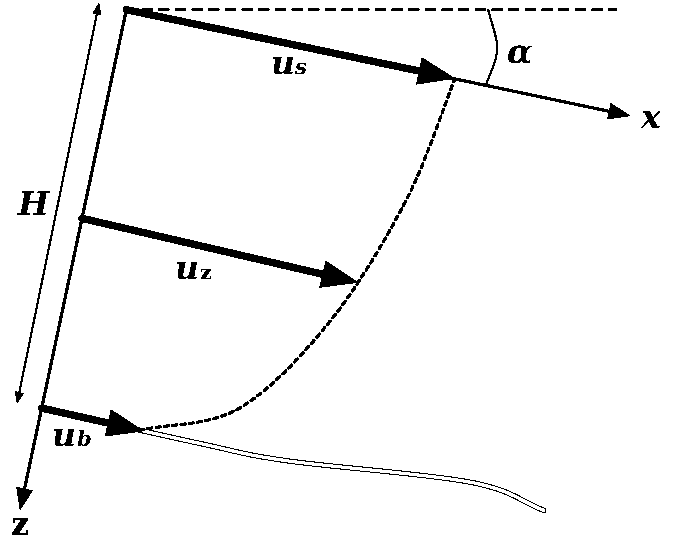
\includegraphics[scale=0.7]{VelocityProfile}
		\caption{Schematic diagram of our velocity profile}
		\label{velocities}
	\end{center}
\end{figure}

By the property $\dot{\epsilon}_{xy} = \frac{1}{2} \left( \frac{\partial u}{\partial y} + \frac{\partial v}{\partial x}\right)$, assuming the shear to take place in the plane normal to $z$ so that $\partial w / \partial x = 0$ and the stress configuration to be of simple shear, the last equation becomes :

\begin{equation}\frac{\mathrm{d} u}{\mathrm{d} z} = 2 \left( \frac{\sigma_{zx}}{B}\right)^n\end{equation}

We can express $\sigma_{zx}$ as a function of $z$ by using the coordinate system of \textsc{Figure} \ref{velocities} and noticing that $\sigma_{zx} = -\rho g h \sin{\alpha}$. After that, integration from the surface to the depth $z$ becomes possible :

\begin{equation}\int_{u_s}^{u(z)} \mathrm{d} u = -2 \left( \frac{\rho g \sin{\alpha}}{B}\right)^n \cdot \int_{0}^{z} z^n \mathrm{d} z\end{equation}


The depth-averaged ice velocity appears after carrying out the integration and rearranging the terms as conducted in \cite{Hooke2005} :

\begin{equation}u(z) = u_s - \frac{2}{n + 1} \left( \frac{\rho g \sin{\alpha}}{B}\right)^n \cdot z^{n+1}\end{equation}

This value becomes computable as soon as we know $u_s$, $B$ and $\alpha$. If we also know the total thickness $H$, the last equation becomes solvable at the bed and we get the bedrock velocity $u_b$ :

\begin{equation}u_b = u_s - \frac{2}{n + 1} \left( \frac{\rho g \sin{\alpha}}{B}\right)^n \cdot H^{n+1}\end{equation}

Our derivation here only is rigorously correct for a slab-shaped glacier of an infinite extent on a uniform slope. If for instance the glacier is bounded laterally, we will have to consider drag on the sides when calculating $\sigma_{zx}$ :

\begin{equation}\sigma_{zx} = -S_f \rho g z \sin{\alpha}\end{equation}

where we have introduced the shape factor $S_f$ ; we possess tables of values for different shapes, but it's good to remember that $S_f$ is $1$ for an infinitely wide glacier, and $\fraction{1}{2}$ for a semicircular glacier.

With that addition, our depth-averaged ice velocity finally reads :

\begin{equation}
\boxed{u(z) = u_s - \frac{2}{n + 1} \left( \frac{S_f \rho g \sin{\alpha}}{B}\right)^n \cdot z^{n+1}}
\end{equation}


\subsection*{The \textit{shallow ice} approximation and theory-motivated velocity}

This approximation concerns large ice sheets where conditions generally vary little over horizontal distances of 5-10 times the local ice thickness \cite{Greve2009}. Ice flow then becomes determined by local conditions such as ice thickness, surface inclination and temperature.
In addition to this, we add some further assumptions :

\begin{itemize}
    \item our bedrock shall be \textit{flat} throughout our measurements
    \item the bedrock shall be frozen, and hence : $u_b = 0$
\end{itemize}

With this basis, the previously derived expression for the base velocity $u_b$ becomes :

\begin{equation}u_b = 0 = u_\circledS - \frac{2}{n + 1} \left( \frac{\rho g \sin{\alpha}}{B}\right)^n \cdot H^{n+1}
\quad
\stackrel{n = 3}{\Longrightarrow}
\quad
\boxed{u_\circledS = \frac{1}{2} \left( \frac{\rho g \sin{\alpha}}{B}\right)^3 \cdot H^4}
\label{GPS:eq:sia}
\end{equation}

where $u_\circledS$ uses the circled subscript for the theory-motivated value of the ice velocity. We will keep using $u_s$ for the sake of generalization, but our theoretical computations in the next chapter will invoke this newly presented $u_\circledS$. 


\subsection*{Calculating the ice flux through an arbitrary cross section profile}

From definition, the ice flux per unit width $q$ is obtained by integrating the velocity profile over depth :

\begin{equation}q = \int_0^H u(z) \, \mathrm{d} z = u_s H - \frac{2}{(n+1)(n+2)} \left( \frac{S_f \rho g \sin{\alpha}}{B}\right)^n \cdot H^{n+2}\end{equation}

Introducing at this stage the mean velocity over depth $\bar{u} \equiv q/H$ reveals to be of greater advantage :

\begin{equation}\bar{u} = u_s - \frac{2}{(n+1)(n+2)} \left( \frac{S_f \rho g \sin{\alpha}}{B}\right)^n \cdot H^{n+1}\end{equation}

From here, after some calculus appears the very ergonomic expression :

\begin{equation}\bar{u} = \frac{4}{5}u_s + \frac{1}{5}u_b = \frac{4}{5}u_\circledS\end{equation}

This last expression allows us to jump back to a formula for the ice flux, reversing the definition of the mean velocity :

\begin{equation}
\boxed{q = \bar{u}H = \frac{4}{5}u_\circledS H}
\end{equation}


\subsection*{Mass balance and the \textit{steady state} assumption}

The massive ice flux per unit width can be defined through :

\begin{equation}q_m = \bar{\rho}q\end{equation}

where $\bar{\rho}$ is the vertically averaged density.

If we define an arbitrary planar cross-section $A$ of width $W$ around the positions where we measured $u_s$, and introduce the mass $M$ of the volume area comprised by $A \cdot H$, then the rate at which it changes would usually be defined \cite{Cuffey2010} by :
 
\begin{equation} \frac{\mathrm{d} M}{\mathrm{d}t} \equiv \bar{\rho} \int_A \dot{b}_i \, \mathrm{d}A - \int_W q_m \, \mathrm{d} W \end{equation}

where $\dot{b}_i$ is the ice-equivalent specific mass balance rate in $\left[ \fraction{m}{yr} \right]$. If we know the direction of the flow, it then becomes easier to pick a arch of width $W$ across the glacier into which $A$ would flow. We shall discover later that this is particularly difficult on both Tellbreen and Blekumbreen, partly because of the small order or magnitude of the measured velocities, which is in accordance with our further theoretical computations, but also because of the quite incoherent positioning over the years of the moving stakes, which makes it impossible to pick a favorite direction for the flux.

Yet if we decide to set the velocity to be zero as a prolongation of our experimental observation and predictions from the theory, then we'd have :

\begin{equation} \frac{\mathrm{d} M}{\mathrm{d}t} \stackrel{u_s = 0}{=} \bar{\rho} \int_A \dot{b}_i \, \mathrm{d}A \end{equation}

In the first order of approximation, should the right-hand side be anything else than zero, this equality would allow us to deny the \textit{steady state} assumption as any non-zero value to be multiplied by $\bar{\rho}$ and integrated over an area $A$ would mean a mass changing rate in the glacier.

\section{Methods and setup} \label{GPS:sec:Methods and setup}
%---Linda

\subsection{Methods}

Regarding to results of the previous years, it is given that the glacier velocity for the glaciers Tellbreen and Blekumbreen is less then one meter.
The general used GPS system has only an accurancy in the order of meters (cite).
This is the reason why we use the differential GPS, which gives a higher accurancy.
By correcting the raw data with the data from the base station, it is posssible to increase the accurancy to the order of millimeters.
The accurancy depends on the distance to the base station (Gölles, 2012) and differs between the horizontal and the vertical component.
The coordinates of the base station ar well known. 
So the disturbances by the atmosphere during the measuring time can be corrected. 
While the post processing the measured coordinates are compare on every timestep defined by the GPS time.
The effect on two measurements at the same postion on two different days are disscussed in the result section.\medskip

The GPS measurements have been done with the Trimble differential Global Navigation Satellite System (GNSS). 
The measured parameters were the northing and easting component as well as the elevation.
The setting during our measurements inculded the receiver Trimble R4, the controller Trimble TCS2 and a carbon pole to mount the receiver proberly next to the stake (see figure).\medskip

During the operation of the measuremts we followed exact the description in section 2 and 3 in Gölles (2012). 
The recommended Fast Static survey method is used.
The used coordinate system is the Universal Transversal Mercator (UTM) for the zone 33x with WGS 1984 date. 
The duration for our measurments with the GPS receiver was at least 15 minutes. 
We had to made choice with a trade off between the quality of the result and the total number of measurements to measure all stakes at least one time. 


\subsection{Setup}

The setup for our measurments is specifed by different guidelines to insure that the measurements are consistent during the whole fieldwork.
The rover on the carbon pole has to be positioned on the top on the stake as far as possible. 
To determine the error from a tilted stake, it is necessary to measure the inclination of the stake as well as the direction of iinclination with the compass.
The snow depth is measured with the probe.
With snow depth and the antenna height the actual elevation on the ice surface is known. 
In addition, the height from the rover above the ice surface is needed to calculate the error by the inclination of the stake.
When the stake is already melted out too high, it is possible to put the pole next to the stake. 
In this case the poles has to be northwards of the stake so that the correction is correlated to only to the northing component. 
Also the distance from rover pole to stake is measured.
For the height and distance measurements the accurancy is one centimeter, because of the one centimeter scale.
The measurement of the inlination with compass has accurancy of two degree caused by the two degree scale.

\begin{figure}
\centering
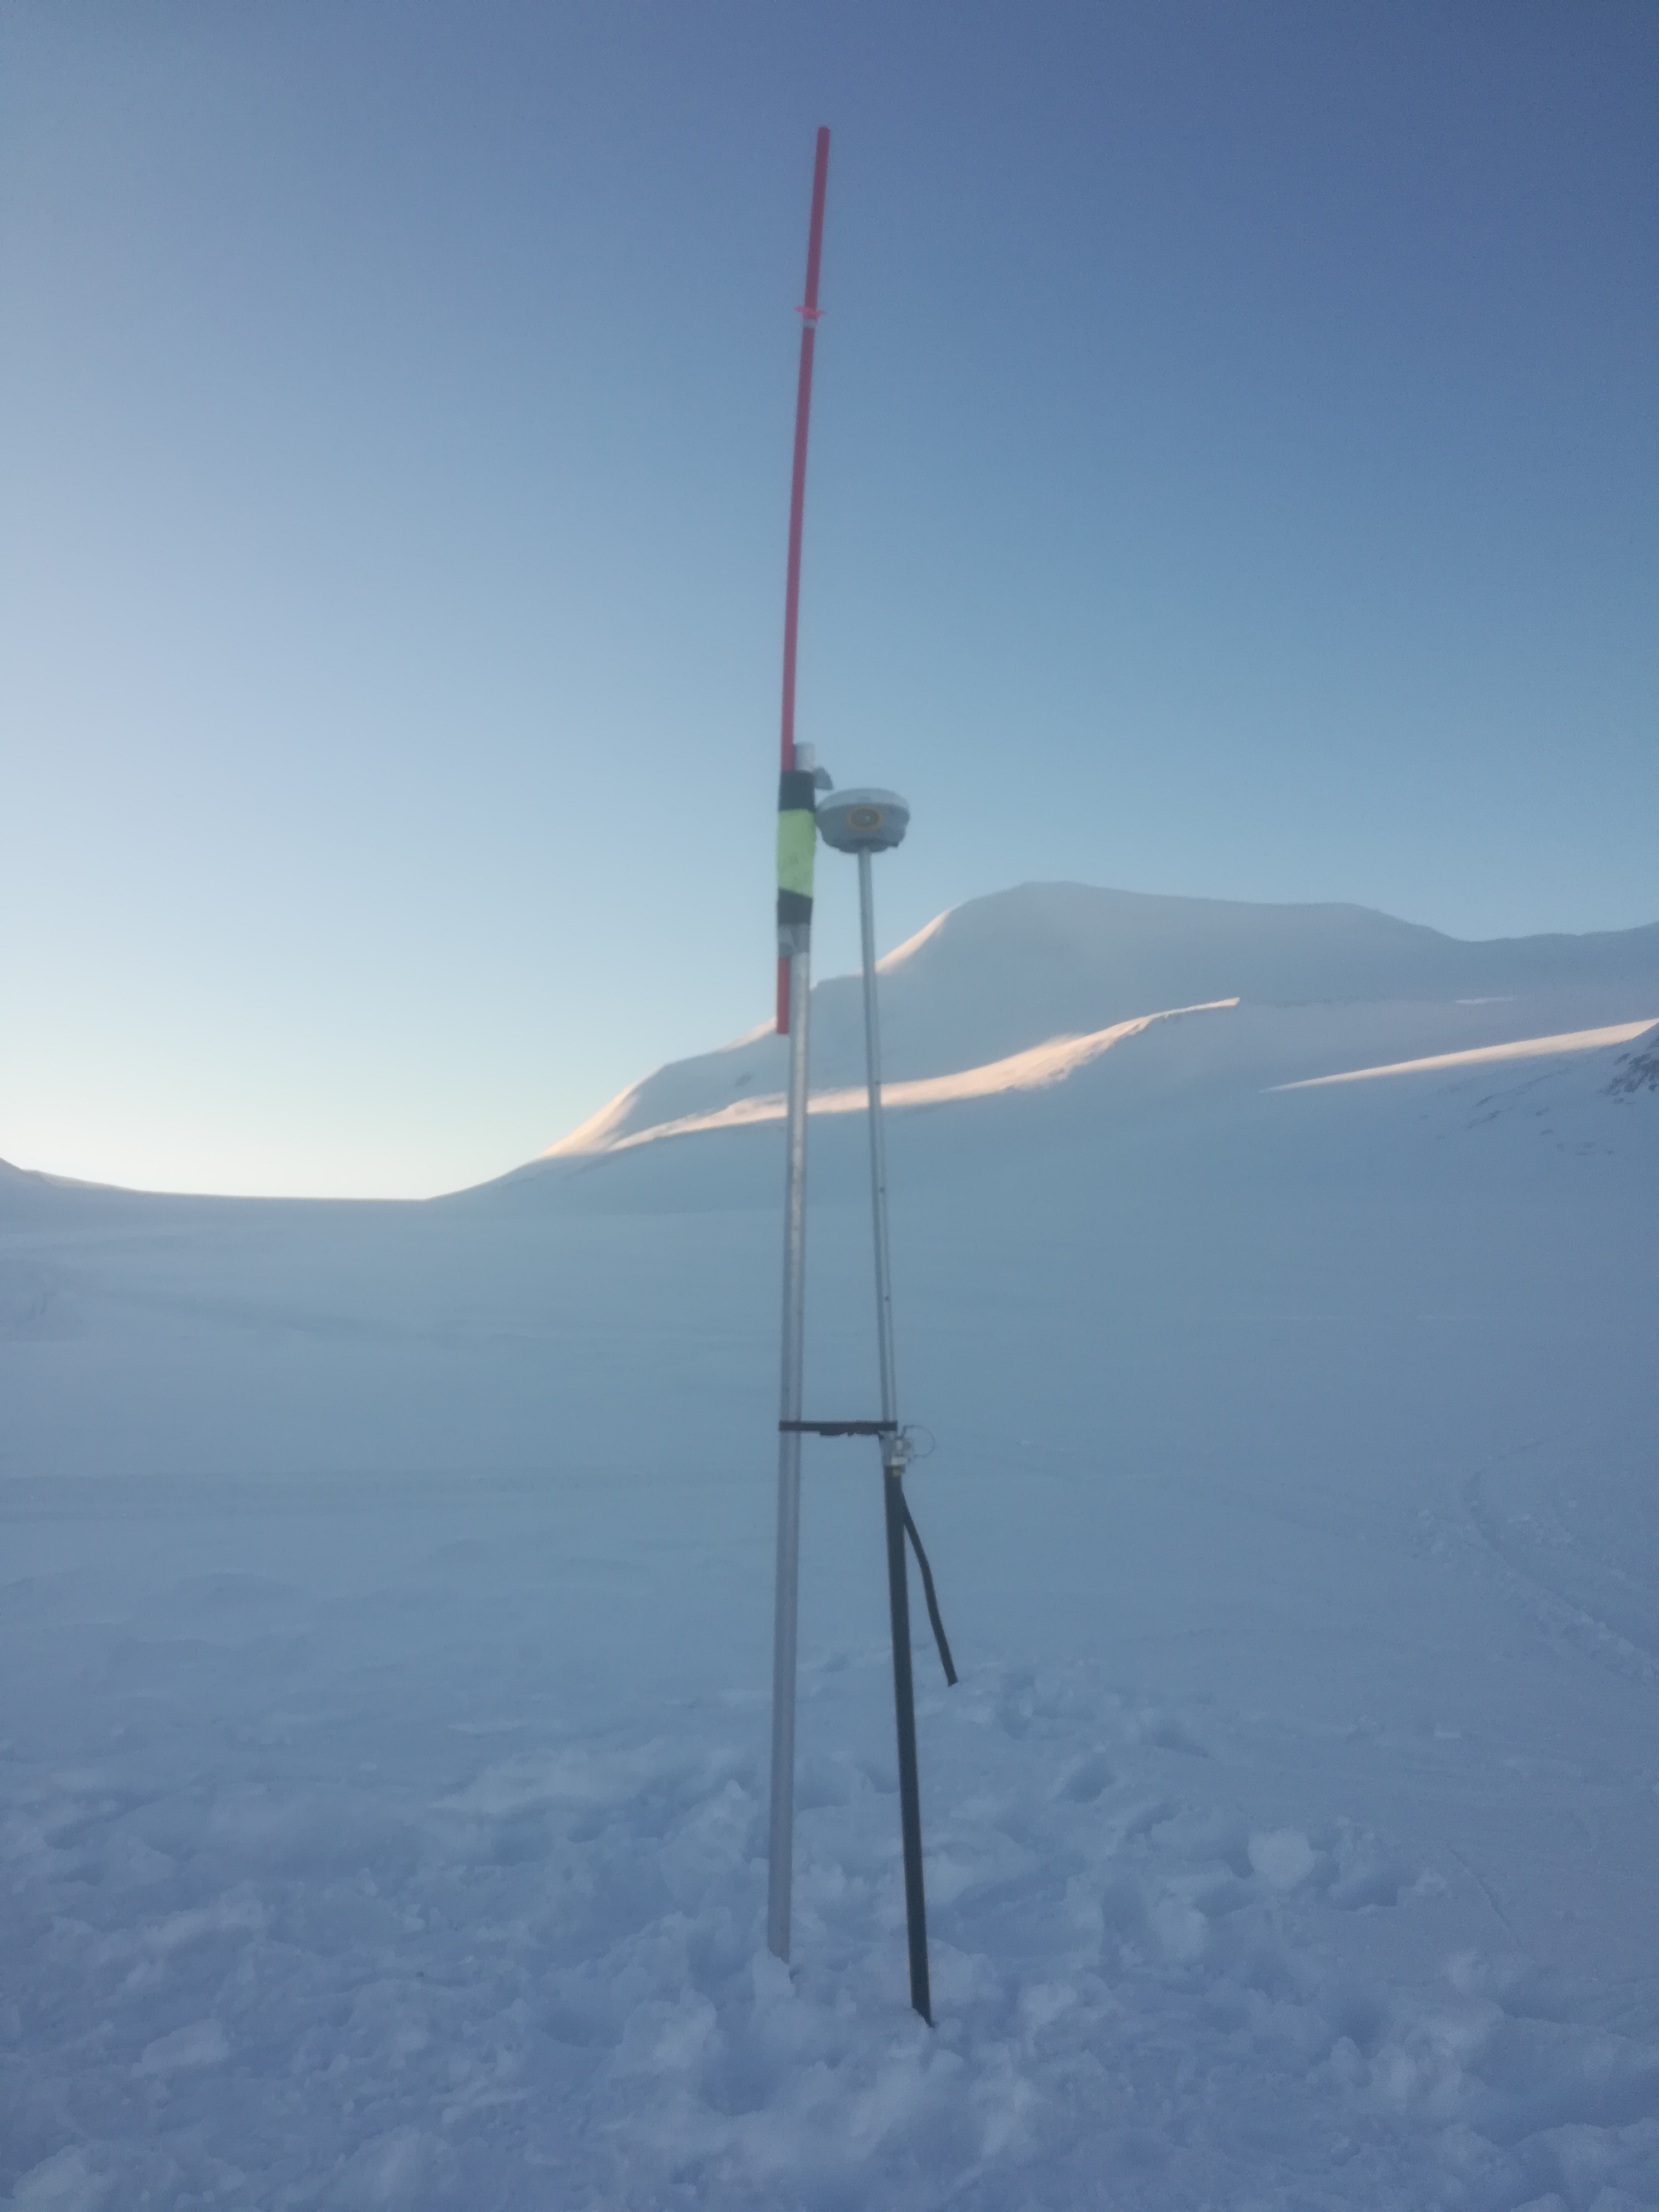
\includegraphics[width=0.48\linewidth]{./figs/pictures/GPS_setup.jpg}
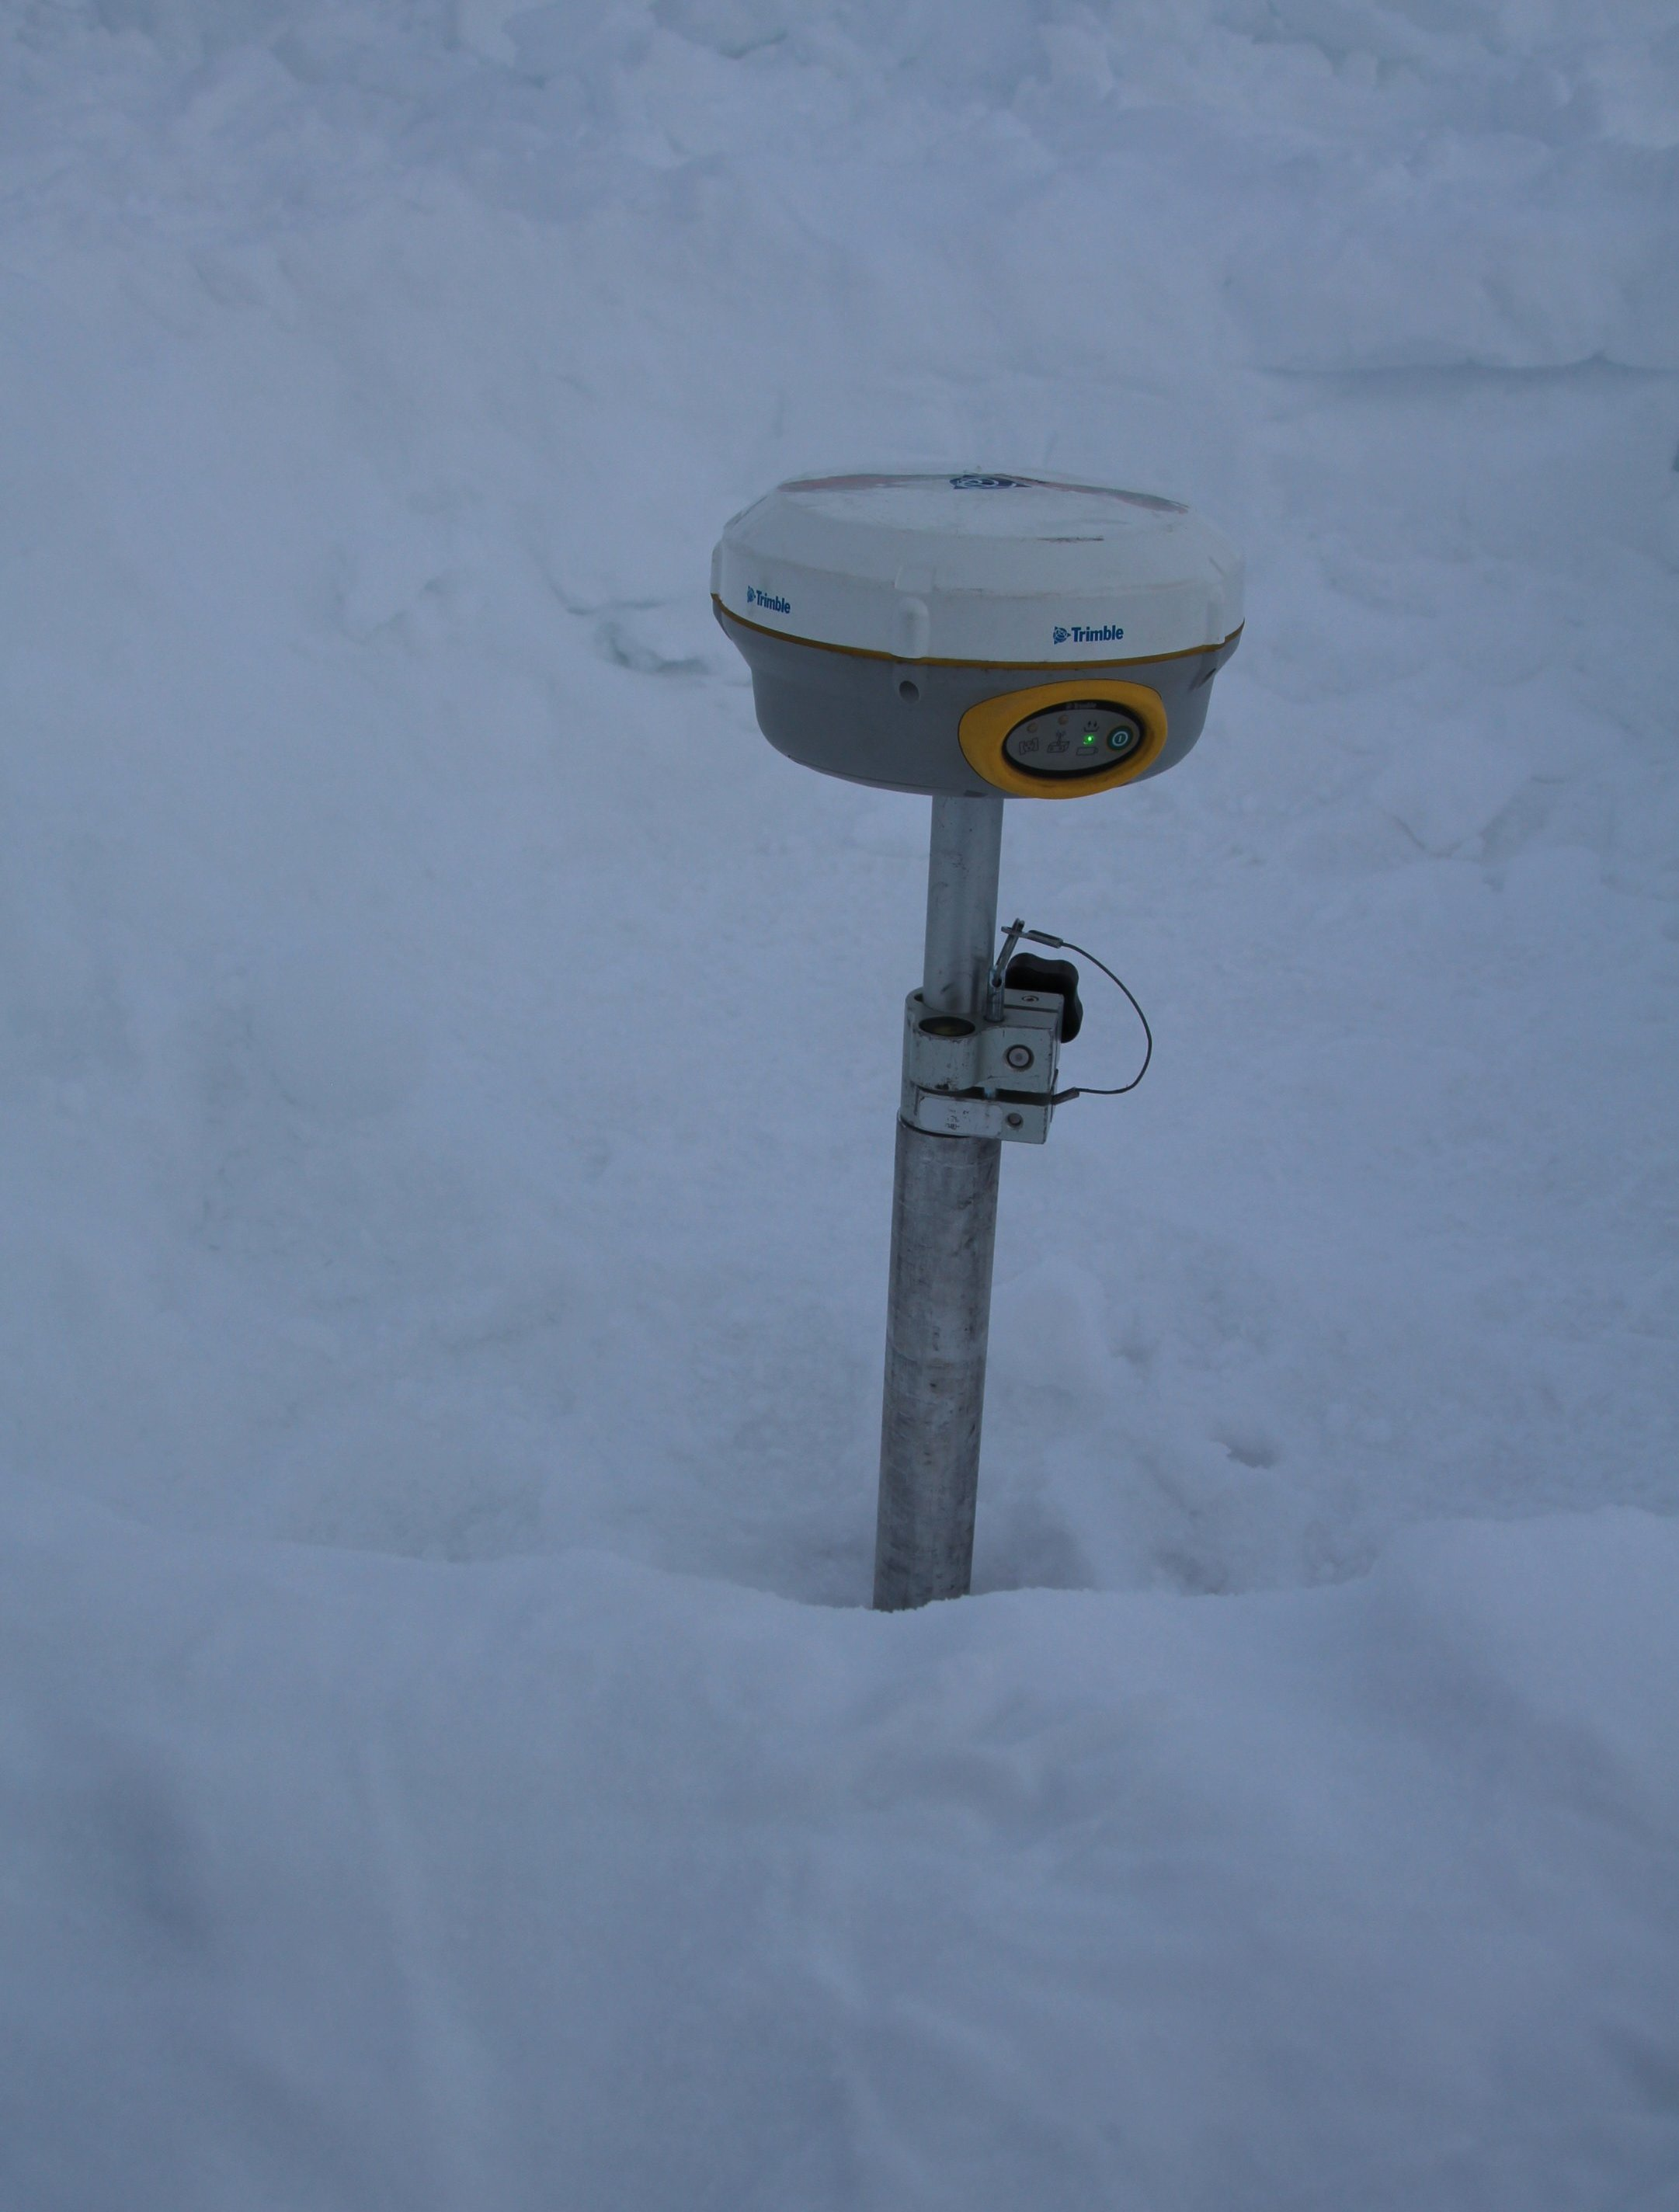
\includegraphics[width=0.485\linewidth]{./figs/pictures/setup_ontop.JPG}
\caption{Setup while the GPS measurement next to the stake (left) and on top of the stake (right).}
\end{figure}


\section{Processing} \label{GPS:sec:Processing}
%---Linda

The post processing is based on the correction of the raw data.
Firstly, we have to process the data with the corresponding data of the base station data to get a higher accurancy of the GPS data.
The nearest base station is Statens Kartverks SatRef located on Platåberget with a distance between 14 km and 20 km depending on the mass balance stake.
In the following the mass balance stake is only named stake and the pole with the rover will be shortend to the name rover.
\medskip

In the previous reports the post processing was done with the commercial software Trimble Business Center (TBC). 
In our report we use a new method for the postprocessing. 
This method is an open source (OS) alternative which is available for different system softwares. 
The TBC is only available on a windows system and needs a licens. 
We operate both methods to compare the results of both methods.
\medskip

\subsection{Trimble}

While the post processing with the usual method in the TBC all steps from section 5 in Gölles (2012) are done.
For each day the data file from the measurements and the corresponding base station data file is imported. 
We have data for the days of year (doy) 070, 072, 074 and 075.
All files from the base station are in the .o18-format. 
The data from the reciever have the .t02 format. 
After the post processing the results from the are stored in a .csv-file.
The GNSS processing in the TBC used the combination of reference and rover data.
The goal is “fix” the number of whole wavelengths between the rover and satellites.
This process is done in two steps by generating a 'float' solution an and resolve an integer value. 
Wheh it is sucessful the solution is defined as 'fixed'.
The transition from 'float' to 'fixed' is the initialization.
A slow convergence of the solution is possible for longer baselines or shielding of the signal by objects in the surrounding.
By mistake it is possible that during the post processing process a wrong fixed values is hold which can lead to an unnormal high position error.
After some amount of time the float solution can switch instantaneously to a fixed solution. 
There is also a disadvantag of the float and fixed approach for integer ambiguity resolution.
At some point in time the convergence to fixed solution is hold on and impossible to change. 
The result define then a wrong position, which is caused by a incorrect set of interger ambiguties.
The TBC use automatically the best way to process the position data. 
It is distingushed in short and long baselines.
Baselines are determined by the distance between rover and reference station.
For longer baselines the errors have to be reduced with an additional approach like a model.
For different settings and situations the TBC used different approaches for the tropospheric and ionospheric errors and choose the right combinaion of different applications.
This makes it difficult to distinguish the settings used for the post processing to compare with the open source processing \citep{Trprocess}.
\medskip

\subsection{Open source}
The OS post processing requires different processing steps.
First of all the raw data file has to be transformed from the original Trimble format .t02 to the .tdg-format, because .t02-files are not readable for the final post processing program.
This transformation was done with the programm runpkr00 which is available on the website of unavco \url{http://kb.unavco.org/kb/article/trimble-runpkr00-v5-40-latest-version-mac-osx-10-7-windows-xp-7-linux-solaris-744.html}.
The used command is 
\begin{verbatim} 
runpkr00 -g -d filename.t02 
\end{verbatim}.
Due to problems with the package we had to do a manual transformation of the package.
To provide the correct file format for the last post processing step we use the toolkit teqc.
This toolkit is also available on the website of unavco \url{https://www.unavco.org/software/data-processing/teqc/teqc.html}.
Then the file can be converted by another commad using
\begin{verbatim}
./teqc +nav filename.nav +obs filename.obs filename.tgd
\end{verbatim} 
to an observation (.obs) and navigation (.nav) file.
After that it is necessary to download also the base station data from the platform \url{http://ftp.statkart.no/}.
The final step in the post processing of the GPS data is done with the open source program package \textit{RTKLIB}.
This package is available for the download in the website \url{http://www.rtklib.com/rtklib.htm}.
In this package we use the executable rtkpost.exe in the subdirectory \textit{/bin} of the downloaded full package with source Programs with the version 2.4.2.
In this software the two navigation file from the receiver and the base station as well as the observation file from the receiver has to be read in.
For this method the .n18-format from the basestation is needed as comparable navigation file.
The next steps are consistent to the description on the website \url{https://docs.emlid.com/reach/common/tutorials/gps-post-processing/}.
For this we had to modify the settings of rtkpost.exe and load the three required files. 
The final output after the post processing is a position file (.pos). 
This file includes for every time step the post processed position in longitude and latitude.
Then we calculate a median over all time steps to get an average position for every measurement.
Because we consistenly use the UTM coordinate system, we transform the lon/lat coordinates by using a python function.
All the analysis in this report is made with python.
\medskip

% therory of the open source post processing
The header with the settings for the OS post processing is available in the appendix.
The setting are as similar as possible to the TBC settings.
But like described is the processing method in the TBC flexible.
In the open source post processing it is possible to select different correction methods for the tropospheric and ionospheric correction. 
Due to missing informations from TBC the probaly best method was choosen with 'broadcast' correction for the ionosphere and the 'saastamoinen' correction for optimize the accurancy due to tropospheric errors. 
The other settings can be taken from the header information to repeat the OS post processing. 
\medskip

The results of the OS post processing are given as a time series of latitude, longitude and elevation, where the horizontal components are transformed to the UTM coordinate system. 
For the better understanding of the OS values it is usefull to compare timeseries of the post processed positions for two different measurements at the same stake.
For both stakes the settings in the post processing were the same.
In the first measurement (figure \label{GPS:fig:T1-i_timeseries}) the values coverge after a few seconds to a fixed solution.
In the second measurement (figure \label{GPS:fig:T1-ii_timeseries}) the values vary during the hole time series.
Out of this time series the weighted average was calculated to get one position value for every stake, the OS value.
The properties of the second measurement leads to a bigger difference between the TBC value and the OS value.
A comparison to the time series of the TBC post processing is not possible, because it is not possible to get this out of the TBC.

\begin{figure}[H]
    \centering
    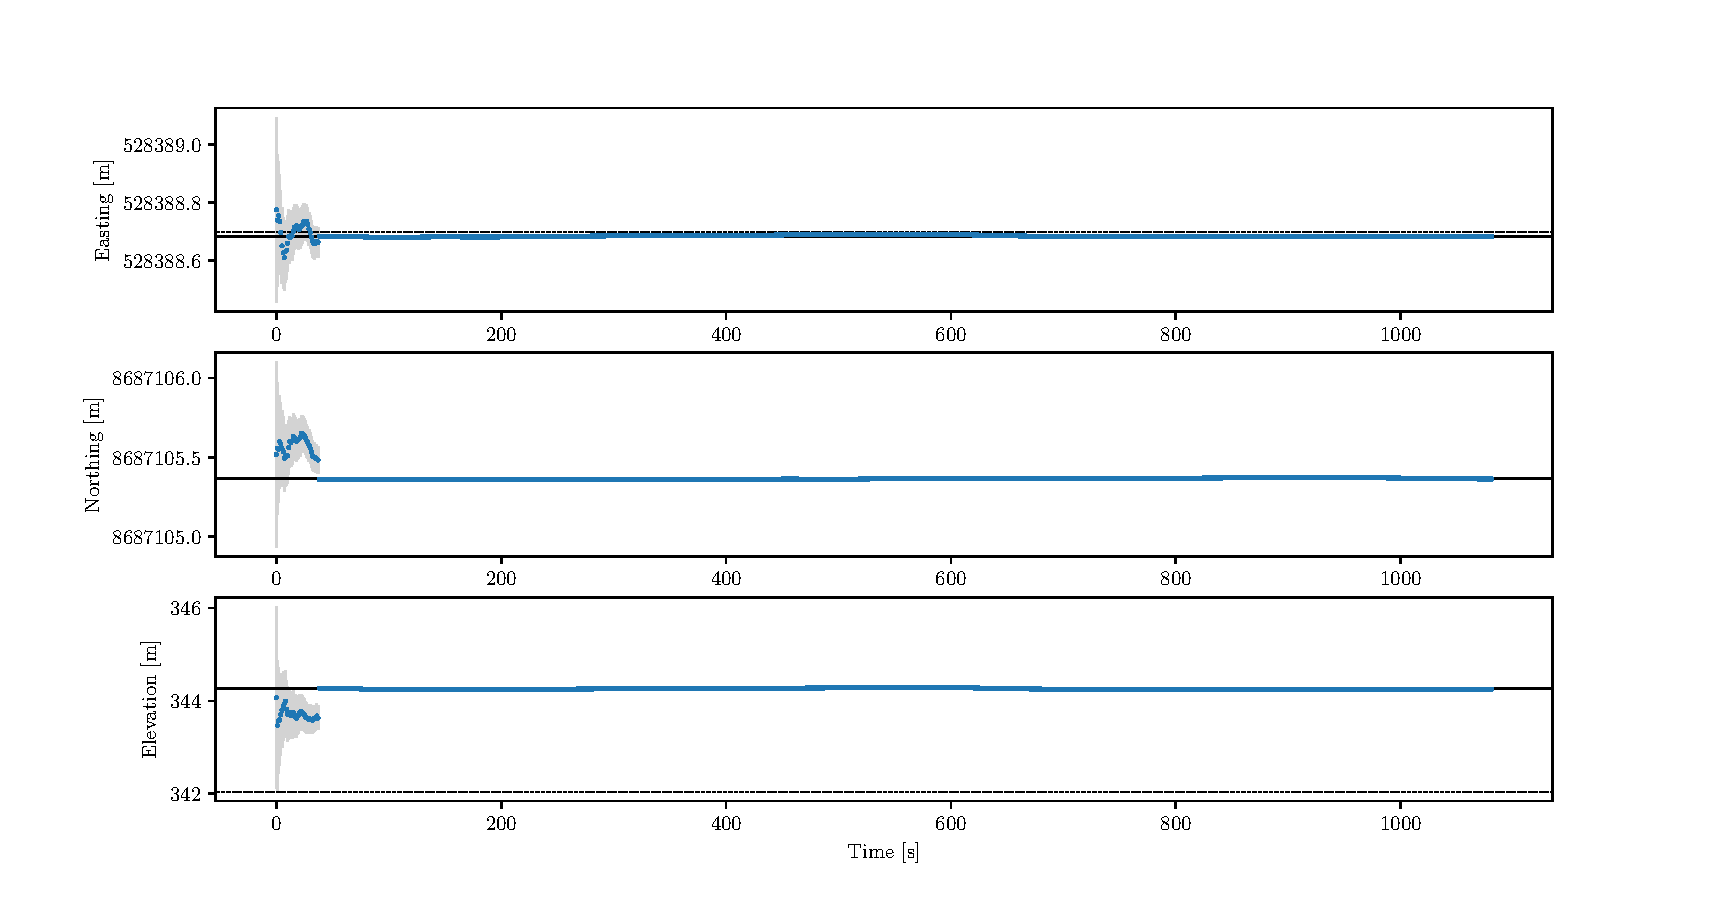
\includegraphics[width=\textwidth]{./figs/timeseries/46250700_corr-T1-i-2017_Timeseries-east-north-elev.pdf}
    \caption{First of two 15 minutes measurements of position of stake T1-2017.}
    \label{GPS:fig:T1-i_timeseries}
\end{figure}

\begin{figure}[H]
    \centering
    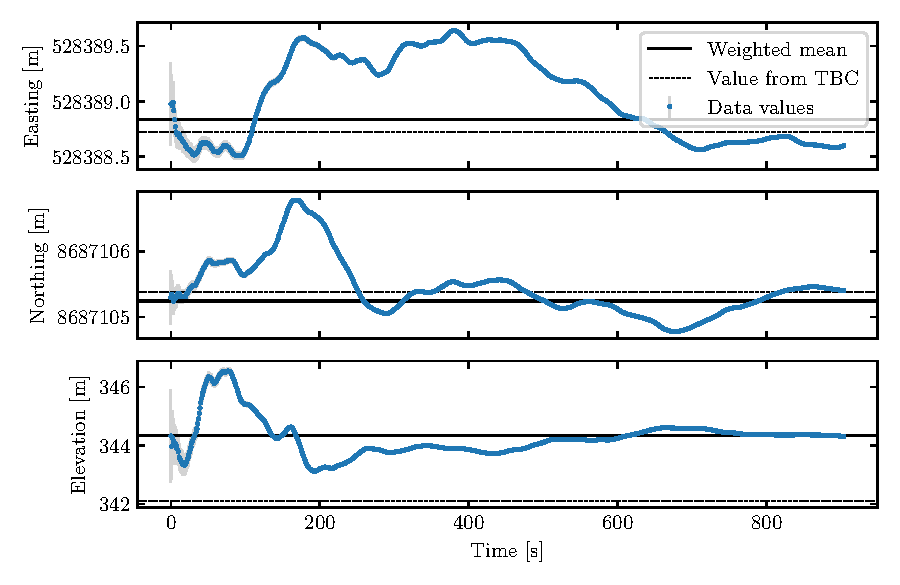
\includegraphics[width=\textwidth]{./figs/timeseries/46250723_corr-T1-ii-2017_Timeseries-east-north-elev.pdf}
    \caption{Second 15 minutes measurement of position of stake T1-2017.}
    \label{GPS:fig:T1-ii_timeseries}
\end{figure}


\subsection{Stake correction}
The post processed data with the base station data are not the final data. 
To get the final, we have to make the stake correction include the different aspects from our measurement setup (see section setup).
We subtract the distance between the rover and the stake from the northing component.
Also it was necessary to correct the position on the ice surface with the inclination of the stake. 
For this, we consider the inclination of the stake and calculate the error dependent on the height of the stake and the direction of the inclination.
The raw data from our measurements which are relevant for our stake corrections are in the appendix in table \ref{GPS:tab:fb_others_tab}.
For the better understanding all variables for the stake corrections are shown in the schematic figure \ref{GPS:fig:schema}.
\medskip

\begin{figure}[H]
	\centering
	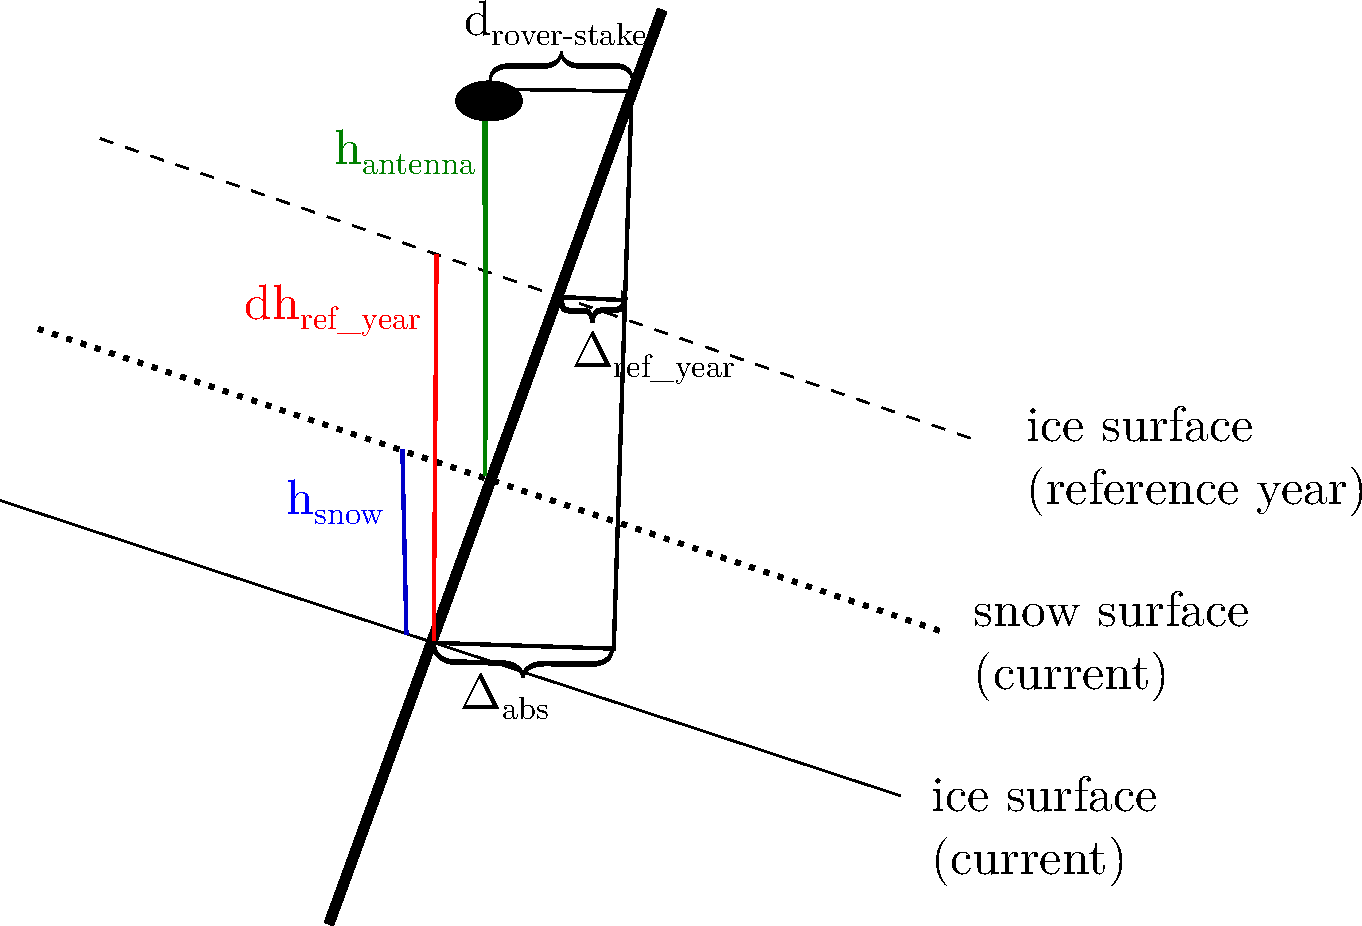
\includegraphics[width=0.9\linewidth]{./figs/pictures/schematic_setup.pdf}
	\caption{Schematic figure of the relevant parameter in the measurment setup.}
	\label{GPS:fig:schema}
\end{figure}

The stake correction is derived by the geomatry of our measurement setup.
First the absolut horizontal difference $\Delta_{\text{abs}}$ depending in the inclination $\alpha$ and the height composite of snow depth $h_{\text{snow}}$ and antenna height $h_{\text{antenna}}$.
\begin{equation}
	\Delta_{\text{abs}} = (h_{\text{snow}} + h_{\text{antenna}}) * sin(\alpha)
\end{equation}

Then the correction is different for the northing and easting. The norting correction is calculated with the cosinus of the direction of the inclination $\phi$. 
The angle of direction is defined in a range from 0$^{\circ}$ to 359$^{\circ}$ with 0$^{\circ}$ for North, 90$^{\circ}$ for East, 180$^{\circ}$ for South and 270$^{\circ}$ for West.
Due to geometrical reasons the sign has to be negative. 
Additionally the the distance between the rover and the stake $d_{\text{rover-stake}}$ has to be subtracted from the original northing.
\begin{equation}
	\Delta_{\text{north}} = - (\Delta_{\text{abs}} * cos(\phi)) - d_{\text{rover-stake}}
\end{equation}

The easting difference $\Delta_{\text{east}}$ is calculated with the sine of $\phi$.
\begin{equation}
	\Delta_{\text{east}} = - \Delta_{\text{abs}} * sin(\phi)
\end{equation}

The elevation correction is different between the OS and the TCS values.
For the TBC values the elevation correction $\Delta_{\text{elev,TBC}}$ only the $h_{\text{snow}}$ need to be subtracted because the $h_{\text{antenna}}$ is already caluclated out while the measurement with the Controller.
\begin{equation}
	\Delta_{\text{elev,TBC}} = - h_{\text{snow}} 
\end{equation}

The elevation correction of the OS elevation $\Delta_{\text{elev,os}}$ is done by $h_{\text{snow}}$ and $h_{\text{antenna}}$.
\begin{equation}
	\Delta_{\text{elev,os}} = - (h_{\text{snow}} + h_{\text{antenna}}) 
\end{equation}

\subsubsection*{Referenced positions}

To calculate the actual velocity it is necessary to reference the location of the stake to the ice surface elevation of the referenced year. 
This has been done for the years 2015, 2016 and 2017 on the 2018 OS values.
In gerneal, the calculation works in the similar way.
The height for stake correction with the inclination is different, because the relevant height difference is, in our case of an over all ablation, lower than for the actual values of this year. So the height difference of the height surface between the referenced year and 2018 $dh_{year,2018}$ is considered for the calculation of the absolute horizontal difference $\Delta_{year,2018}$.

\begin{equation}
	\Delta_{year,2018} = (h_{\text{snow}} + h_{\text{antenna}} - dh_{year,2018}) * sin(\alpha)
\end{equation}

\subsection{Evaluation}

For the difference between the two different methods is not systematic and in the avereage of the absolute values in the order of centimeters with 0.09 m for the northing, 0.05 m for thehe  easting and 0.24 m for the elevation. This is mainly caused by a few unclear values after the post processing. The meadian of the northing and eastind difference is about 0.01 m and for the elevation only 0.07 m. For the comparison the TBC post processed coordinates are in the appendix in table \ref{GPS:tab:tbc_tab}.
The differences for northing, easting and elevation for every stake is displayed in a table in the appendix in table \ref{GPS:tab:diff_tab}. 

This shows that the OS processed values are a reasonable replacement for the TBC values.
This means that in the following report the OS values are consideres.
This means also that the error propagation is done for the OS values so we can finaly determine the uncertainty of the velocity values.

\subsection{Error propagation}

The calculations for the error propagation are done by following the common rule.
The accurancy of the post processed postions with the base station data is decreasing with a increasing distance to the base station. 
But this error is at least one order of magnitude smaller than the other errors. 
The other accurancies are determined by the quality of our measurements \ref{GPS:tab:errors}.

\begin{table}[H]
	\caption{Used error values for the error propagation.}
	\centering
	\begin{tabular}{lc}
	\toprule
        error &  value \\
	\midrule
    $ \delta_{\alpha} $ &  3$^{\circ}$ \\
    $ \delta_{\phi} $ &  22.5$^{\circ}$ \\
    $ \delta_{h_{snow}}$ &  0.02 m \\
    $ \delta_{h_{antenna}} $ &  0.05 m \\
    $ \delta_{dh_{year,2018}} $ &  0.10 m \\
    $ \delta_{d_{rover-stake}} $ &  0.02 m \\
    $ \overline{\delta_{\Delta_{north}}} $ & 0.40 m \\
    $ \overline{\delta_{\Delta_{east}}} $ & 0.19 m \\
    $ \overline{\delta_{\Delta_{elev}}} $ & 0.89 m \\
    \bottomrule
	\end{tabular}
	\label{GPS:tab:errors}
\end{table} 

The error calculation for the final position is dependent of different errors.

The error of the absolut horizontal difference $\delta_{\Delta_{\text{abs}}}$ is dependent on the errors of the parameter and the parameter itself.
\begin{equation}
	\delta_{\Delta_{\text{abs}}} = \sqrt{(h_{\text{snow}} + h_{\text{antenna}})^2 * \delta_{\alpha}^2 * cos^2(\alpha) + (\delta_{h_{\text{snow}}}^2 + \delta_{h_{\text{antenna}}}^2) * \sin^2(\alpha)}
\end{equation}

The error of the northing correction $\delta_{\Delta_{\text{north}}}$ is
\begin{equation}
	\delta_{\Delta_{\text{north}}} = \sqrt{\delta_{\Delta_{\text{abs}}}^2 * cos^2(\phi) + \Delta_{\text{abs}}^2 * \delta_{\phi}^2 * sin^2(\phi) + \delta_{d_{\text{rover-stake}}}^2}
\end{equation}

The error of the easting correction $\delta_{\Delta_{\text{east}}}$ is
\begin{equation}
	\delta_{\Delta_{\text{east}}} = \sqrt{\delta_{\Delta_{\text{abs}}}^2 * sin^2(\phi) + \Delta_{\text{abs}}^2 * \delta_{\phi}^2 * cos^2(\phi)}
\end{equation}

The error of the elevation correction $\delta_{\Delta_{\text{elev}}}$ is
\begin{equation}
\delta_{\Delta_{\text{elev}}} = \sqrt{\delta_{h_{\text{snow}}}^2 + \delta_{h_{\text{antenna}}}^2}
\end{equation}
	
Based on this errors the total error for norting $\delta_{\Delta_{\text{total,north}}}$, easting $\delta_{\Delta_{\text{total,east}}}$ and eleavtion $\delta_{\Delta_{\text{total,elev}}}$ can calculated with the error of the time series of our OS post processed GPS time series $\delta_{\Delta_{\text{ts,north}}}$ for northing, $\delta_{\Delta_{\text{ts,east}}}$ for easting and $\delta_{\Delta_{\text{ts,elev}}}$ for the elevation.
\begin{equation}
	\delta_{\Delta_{\text{total,north}}} = \sqrt{\delta_{\Delta_{\text{ts,north}}}^2 + \delta_{\Delta_{\text{north}}}^2}
\end{equation}

\begin{equation}
	\delta_{\Delta_{\text{total,east}}} = \sqrt{\delta_{\Delta_{\text{ts,east}}}^2 + \delta_{\Delta_{\text{east}}}^2}
\end{equation}

\begin{equation}
	\delta_{\Delta_{\text{total,elev}}} = \sqrt{\delta_{\Delta_{\text{ts,elev}}}^2 +\delta_{\Delta_{\text{elev}}}^2}
\end{equation}

\subsubsection*{Referenced positions}
For the refenced positions only two euations differ to the previous error propagation. 
The error of the absolute difference $\Delta_{year,2018}$ is
\begin{equation}
\begin{split}
\delta_{\Delta_{year,2018}} = & 
\ ((h_{\text{snow}} + h_{\text{antenna}} - dh_{year,2018})^2 * \delta_{\alpha}^2 * cos^2(\alpha)\\
&+ (\delta_{h_{\text{snow}}}^2 + \delta_{h_{\text{antenna}}}^2 + \delta_{dh_{year,2018}}^2) * \sin^2(\alpha))^{1/2}
\end{split}
\end{equation}

The error for the elevation correction $\delta_{\Delta_{year, \text{elev}}}$ is also different by the uncertainty of the height difference of the ice surface $\delta_{dh_{\text{year, 2018}}}$.
\begin{equation}
	\delta_{\Delta_{year, \text{elev}}} = \sqrt{\delta_{h_{\text{snow}}}^2 + \delta_{h_{\text{antenna}}}^2 + \delta_{dh_{\text{year, 2018}}}^2}
\end{equation}

\subsection{Final positions}

The final data with all the processing and correction included show the actual position of the stakes on this years ice surface.

\begin{table}[H]
	\caption{Final positions after the open source post processing and stake correction with the error.}
	\centering
	\begin{tabular}{lrrrrrr}
\toprule
        Name &  Northing [m] &  Error Northing [m] &  Easting [m] &  Error Easting [m] &  Elevation [m] &  Error Elevation [m] \\
\midrule
    BL2-2016 &    8686150.74 &                0.16 &    523049.41 &               0.11 &         436.89 &                 0.48 \\
    BL2-2018 &    8686149.82 &                0.01 &    523051.47 &               0.03 &         437.74 &                 0.06 \\
    BL3-2016 &    8686091.51 &                0.27 &    523544.75 &               0.13 &         490.82 &                 0.25 \\
    BL3-2018 &    8686091.17 &                0.42 &    523545.34 &               0.10 &         491.39 &                 1.03 \\
    BL4-2018 &    8686098.58 &                0.17 &    524179.27 &               0.15 &         573.74 &                 0.20 \\
  BL4-i-2016 &    8686098.47 &                0.26 &    524179.80 &               0.19 &         571.65 &                 0.20 \\
 BL4-ii-2016 &    8686098.39 &                1.30 &    524179.92 &               0.31 &         571.36 &                 4.82 \\
  BL5-i-2017 &    8686130.74 &                0.09 &    524644.27 &               0.01 &         628.63 &                 0.09 \\
 BL5-ii-2017 &    8686130.74 &                0.28 &    524644.28 &               0.15 &         628.56 &                 0.75 \\
     T1-2018 &    8687106.55 &                0.32 &    528388.42 &               0.07 &         341.59 &                 0.24 \\
   T1-i-2017 &    8687105.69 &                0.13 &    528388.68 &               0.18 &         341.26 &                 0.12 \\
  T1-ii-2017 &    8687105.58 &                0.45 &    528388.84 &               0.44 &         341.38 &                 0.65 \\
     T2-2016 &    8687321.31 &                0.42 &    527951.88 &               0.14 &         394.88 &                 2.34 \\
     T2-2018 &    8687319.62 &                0.28 &    527951.35 &               0.27 &         395.86 &                 1.61 \\
   T2-i-2017 &    8687321.37 &                0.30 &    527950.58 &               0.25 &         395.22 &                 0.34 \\
  T2-ii-2017 &    8687320.98 &                1.31 &    527951.01 &               0.26 &         394.74 &                 1.26 \\
     T3-2017 &    8687273.11 &                0.11 &    527598.29 &               0.01 &         422.59 &                 0.07 \\
     T4-2016 &    8687138.56 &                0.47 &    527123.97 &               0.34 &         486.80 &                 1.07 \\
     T4-2018 &    8687137.72 &                1.05 &    527124.90 &               0.37 &         487.94 &                 2.33 \\
     T5-2016 &    8686938.28 &                0.57 &    526692.25 &               0.25 &         534.57 &                 0.72 \\
     T5-2018 &    8686937.68 &                0.21 &    526690.76 &               0.21 &         535.09 &                 0.45 \\
     T6-2016 &    8686675.01 &                0.51 &    526250.17 &               0.22 &         561.87 &                 0.89 \\
     T6-2018 &    8686674.78 &                0.48 &    526246.88 &               0.39 &         560.47 &                 0.79 \\
     T7-2015 &    8686578.89 &                0.24 &    525858.01 &               0.17 &         615.10 &                 0.71 \\
     T7-2017 &    8686579.37 &                0.19 &    525858.38 &               0.04 &         615.95 &                 0.71 \\
     T8-2017 &    8686471.52 &                0.48 &    525523.82 &               0.13 &         649.73 &                 1.02 \\
\bottomrule
\end{tabular}

	\label{GPS:tab:os_tab}
\end{table}


\section{Results} \label{GPS:sec:Results}
\subsection{Horizontal velocity (ice flow)}

\begin{figure}[H]
    \centering
    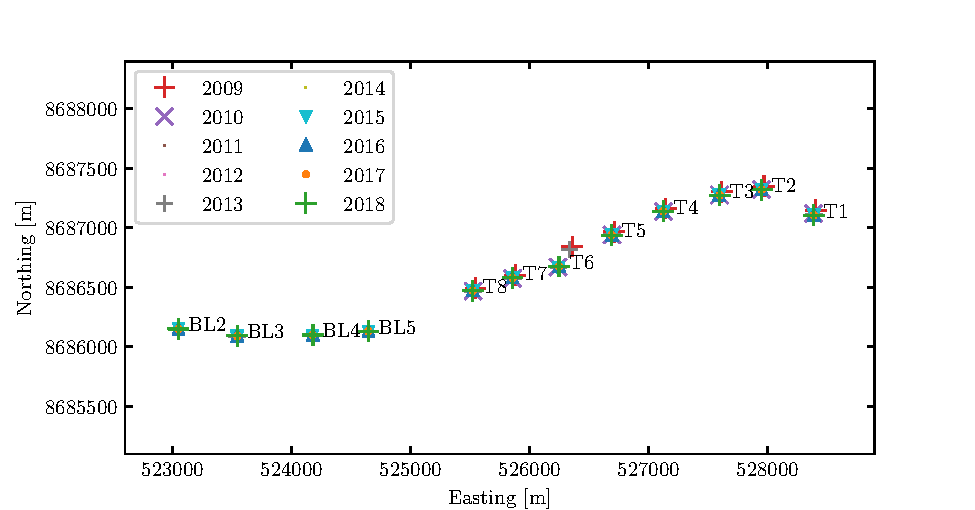
\includegraphics[width=\textwidth]{./figs/stakePositions.pdf}
    \caption{Positions of all stakes in the flow line on Blekumbreen and Tellbreen.
    The different markers distinguish the year of the measurement.}
    \label{GPS:fig:stakepos}
\end{figure}

Figure~\ref{GPS:fig:stakepos} shows the positions of the currently 12 different stake locations
on Blekumbreen and Tellbreen.
At those locations, a total of 26 measurements has been performed in 2018.
Additionally, all available data of the stake positions since 2009 is shown on the figure.\\
The coarse resolution of the figure shows a rough accordance of all of this year's positions with the values 
of the last years.
The stakes spread over about 5 kilometers in east-west direction and 1.5 kilometers in north-south direction.

Figure~\ref{GPS:fig:T1_2d} shows all available data for one single stake (T1) in a higher resolution.\\
The measurement of the location of T1-2017 (green) has been performed two times
(see Figures~\ref{GPS:fig:T1-i_timeseries} and \ref{GPS:fig:T1-ii_timeseries})
in order to estimate the uncertainty
of the position.
The two positions differ by 19\,cm and match within their uncertainties.

Equation~\ref{GPS:eq:v} gives the relation how the ice velocity $v_{year}$ has been calculated from the corrected stake positions in
Tab.~\ref{GPS:tab:os_tab}:
The distance between this year's position and the position measured in 2017, 2016 or 2015 has been divided
by the passed time $t$ (1, 2 or 3 years).
$N_{year}$ and $E_{year}$ are the northing and easting of the year which has been used to calculate the distance to
this year's position.
The positions of this year ($N_{year, 2018}$ and $E_{year, 2018}$) have been shifted by the respective distance
$\Delta_{\text{ref}, year}$ that ablation has
added to inclined stakes since the year $year$, as described in section~\ref{GPS:sec:Processing}.
Equation~\ref{GPS:eq:sv} shows how the error on $v_{year}$ has been obtained.
For the uncertainties on the past year's values ($\delta_{N_{year}}^2$ and $\delta_{E_{year}}^2$),
the mean uncertainties $\overline{\delta_{\text{N}}}$ and $\overline{\delta_{\text{E}}}$ of this year's values
from Tab~\ref{GPS:tab:errors} have been used.

Table~\ref{GPS:tab:vel_tab} lists the calculated velocities for all stakes.
The direction of the movements can be seen on the detailed figures for each stake in the appendix.


\begin{figure}[htb]
    \centering
    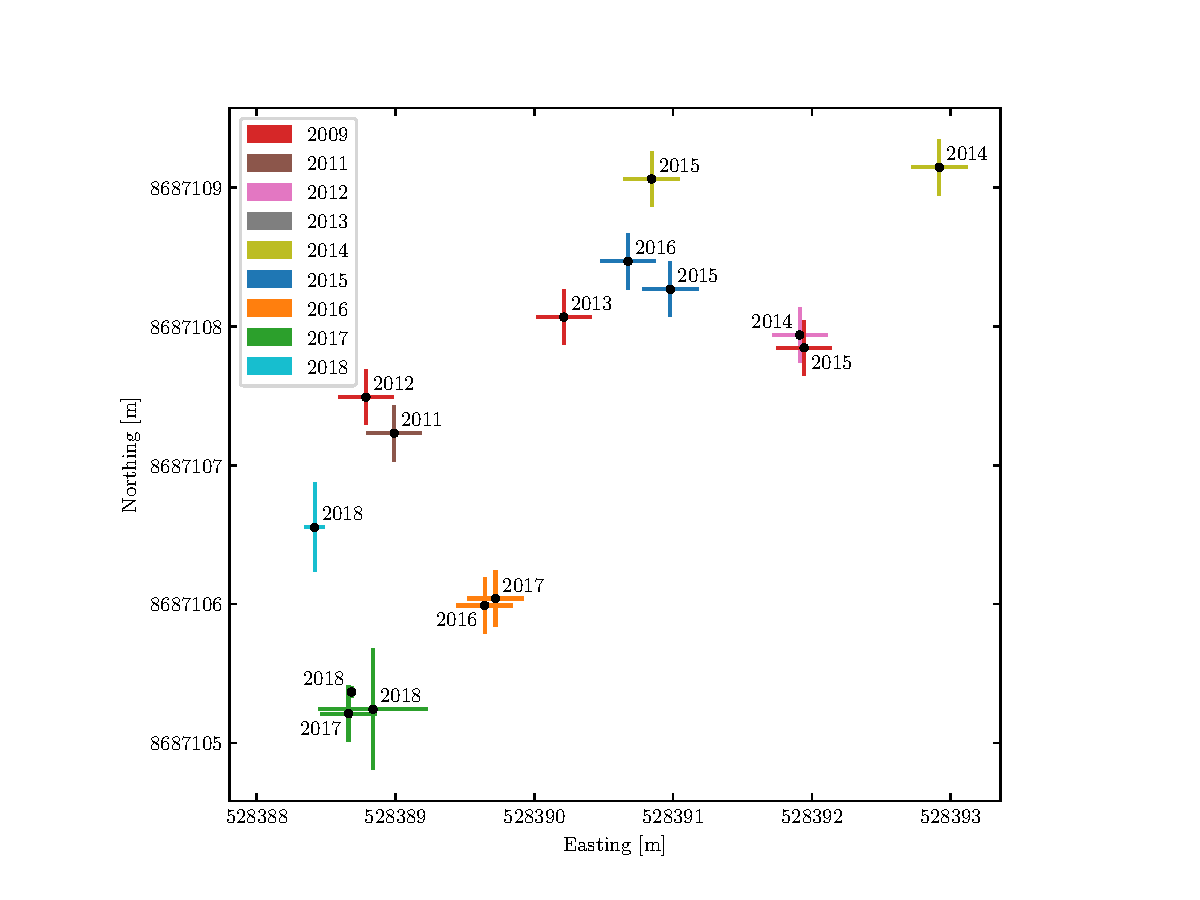
\includegraphics[width=\textwidth]{./figs/T1_2d.pdf}
    \caption{Measured positions at the location of stake T1 from 2011 to 2018.
    Different colors denote different stakes;
  	the year next to each stake position is the year of the measurement.
  	The measurements of 2018 have been corrected by the inclination of the stake and
  	the distance between the stake and the rover, therefore the coordinates refer to the intersection point
  	of stake and glacier surface.
    	At this location, a movement in south-east direction would be expected.
    	This is not identifiable using the data at hand.
 	Similar plots of the other 11 stake locations are situated in the appendix.}
    \label{GPS:fig:T1_2d}
\end{figure}


\begin{table}[htb]
	\caption{Velocities of the stakes measured in 2018, calculated with equations~\ref{GPS:eq:v} and \ref{GPS:eq:sv}.
	The velocity $v_{2017}$ has been calculated using last year's position.
	For inclined stakes, this position has been corrected for the horizontal displacement due to ablation.
	If available, corrected positions from 2016 and 2015 have also been used to obtain $v_{2016}$ and $v_{2015}$.
	To be able to assess the uncertainty of the velocities, four measurements have been performed twice.
	This is denoted by the subscripts -i and -ii.}
	\centering
	\begin{tabular}{lcccccc}
\toprule
  Stake name & Velocity (2017) [m/a] & Velocity (2016) [m/a] & Velocity (2015) [m/a] \\
\midrule
    BL2-2016 &       0.26 $\pm$ 0.21 &       0.21 $\pm$ 0.20 &                     - \\
    BL3-2016 &       0.16 $\pm$ 0.20 &       0.21 $\pm$ 0.18 &                     - \\
  BL4-i-2016 &       0.07 $\pm$ 0.26 &       0.08 $\pm$ 0.25 &                     - \\
 BL4-ii-2016 &       0.11 $\pm$ 0.56 &       0.05 $\pm$ 0.48 &                     - \\
  BL5-i-2017 &       1.75 $\pm$ 0.18 &                     - &                     - \\
 BL5-ii-2017 &       1.74 $\pm$ 0.24 &                     - &                     - \\
   T1-i-2017 &       0.09 $\pm$ 0.11 &                     - &                     - \\
  T1-ii-2017 &       0.19 $\pm$ 0.43 &                     - &                     - \\
     T2-2016 &       0.60 $\pm$ 0.24 &       0.28 $\pm$ 0.20 &                     - \\
   T2-i-2017 &       0.23 $\pm$ 0.30 &                     - &                     - \\
  T2-ii-2017 &       0.53 $\pm$ 0.51 &                     - &                     - \\
     T3-2017 &       0.10 $\pm$ 0.12 &                     - &                     - \\
     T4-2016 &       0.13 $\pm$ 0.38 &       0.17 $\pm$ 0.37 &                     - \\
     T5-2016 &       0.30 $\pm$ 0.33 &       0.12 $\pm$ 0.22 &                     - \\
     T6-2016 &       0.79 $\pm$ 0.31 &       0.12 $\pm$ 0.19 &                     - \\
     T7-2015 &       0.26 $\pm$ 0.27 &       0.10 $\pm$ 0.15 &       0.08 $\pm$ 0.19 \\
     T7-2017 &       1.33 $\pm$ 0.16 &                     - &                     - \\
     T8-2017 &       0.20 $\pm$ 0.24 &                     - &                     - \\
\bottomrule
\end{tabular}

	\label{GPS:tab:vel_tab}
\end{table}

\begin{equation}
\label{GPS:eq:v}
v_{year} = \frac{\sqrt{(N_{year, 2018}-N_{year})^2+(E_{year, 2018} - E_{year})^2}}{t}
\end{equation}

\begin{equation}
\label{GPS:eq:sv}
\delta_{v_{year}} = \sqrt{\frac{
(\delta_{N_{year, 2018}}^2 + \delta_{N_{year}}^2) * (N_{year, 2018}-N_{year})^2 +
(\delta_{E_{year, 2018}}^2 + \delta_{E_{year}}^2) * (E_{year, 2018}-E_{year})^2}
{(N_{year, 2018} - N_{year})^2+ (E_{year, 2018} - E_{year})^2}}
\end{equation}


\subsection{Vertical velocity (mass balance)} \label{GPS:subsec:maba}

Besides the horizontal position, the GPS data also contain elevation.
An analysis of the change of elevation (the vertical velocity) of the stakes over the past years offers the possibility to determine the individual average mass balances.\\
We have been able to find elevation data from former groups for the last 7 years,
back until 2011.
Figures~\ref{GPS:fig:elev_ble} and \ref{GPS:fig:elev_tel} show this data,
together with the new data from 2018.
For most of the old data points, the uncertainties are not known.
Therefore there are no error bars shown on the plots.

Apart from a couple of outliers, the elevation of all stakes decreases quite linearly.
Therefore linear fits of the elevation have been performed for all stakes individually.
The results of the fits are shown in Tables~\ref{GPS:tab:mbal_ble} and \ref{GPS:tab:mbal_tel}.\\
With the individual mass balances for each stake,
it is possible to calculate the mass balance gradients and the equilibrium line elevations of the two glaciers.
This is shown in Figs.~\ref{GPS:fig:elev_ble_mbg} and \ref{GPS:fig:elev_tel_mbg}.
The values on the y-axis (stake elevation) are mean values of all elevation measurements of the different years.

The linear fits yield the following results for the equilibrium lines (EL) and mass balance gradients~(MBG) on Blekumbreen and Tellbreen:
\begin{equation*}
\begin{split}
\text{EL}_\text{B} = 751 \pm 45\, \text{m} \qquad \text{MBG}_\text{B} = 5.1 \pm 1.0\, \text{mm/m}\\
\text{EL}_\text{T} = 757 \pm 56\, \text{m} \qquad \text{MBG}_\text{T} = 6.8 \pm 1.4\, \text{mm/m}
\end{split}
\end{equation*}


\begin{figure}[htb]
    \centering
    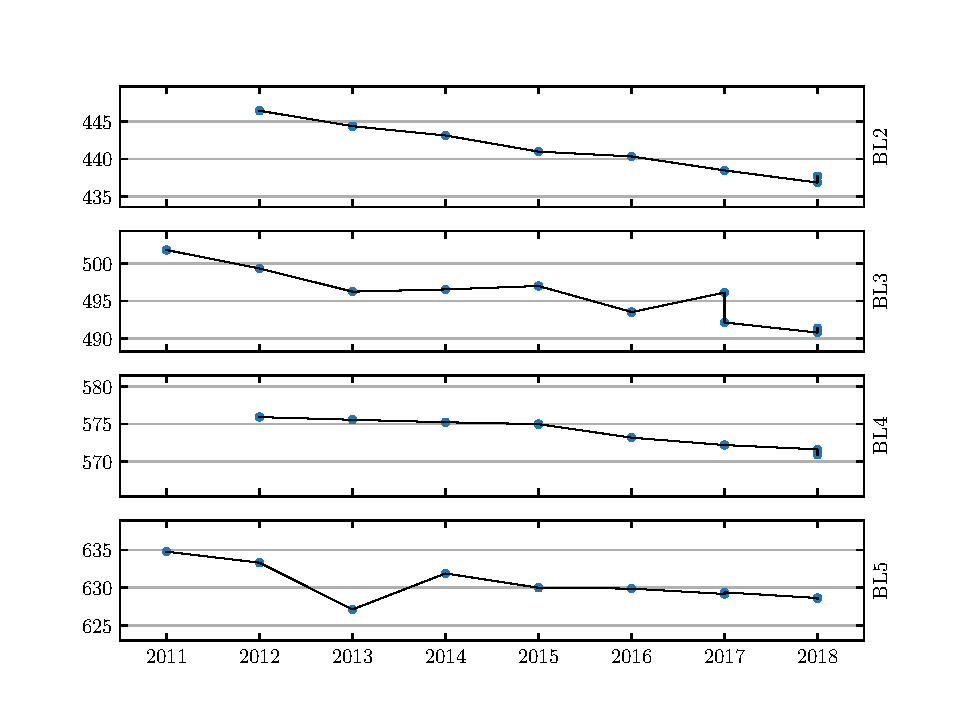
\includegraphics[width=\textwidth]{./figs/Elevation_Blekumbreen.pdf}
    \caption{GPS measured elevation of the stakes on Blekumbreen from 2011 until 2018 (blue dots).
    Linear fits (red line) of the data have been performed to calculate the individual mass balances~$b$.}
    \label{GPS:fig:elev_ble}
\end{figure}


\begin{figure}[htb]
    \centering
    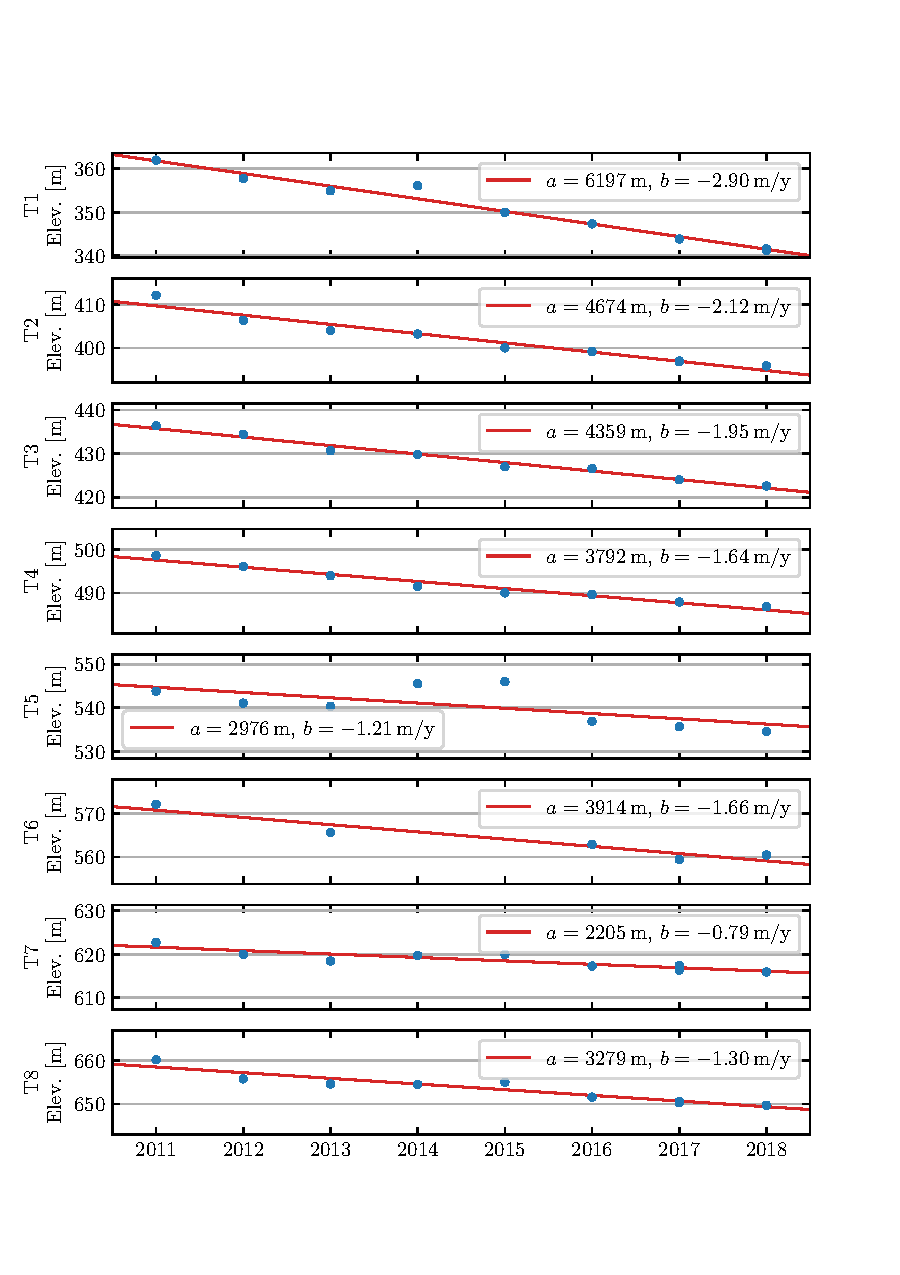
\includegraphics[width=\textwidth]{./figs/Elevation_Tellbreen.pdf}
    \caption{GPS measured elevation of the stakes on Tellbreen from 2011 until 2018 (blue dots).
    Linear fits (red line) with $y = a + x*b$ have been performed to calculate the individual mass balances~$b$.}
    \label{GPS:fig:elev_tel}
\end{figure}

\begin{table}[htb]
	\caption{Mass balance as result of the elevation fits from Fig.~\ref{GPS:fig:elev_ble} and
	mean values of the elevation measurements for all stakes on Blekumbreen.
    The data in the table is plotted in Fig.~\ref{GPS:fig:elev_ble_mbg}.}
	\centering
	\begin{tabular}{lcc}
\toprule
Stake name & Elevation [m] &  Mass balance [m] \\
\midrule
       BL2 &         441.7 &  -1.45 $\pm$ 0.08 \\
       BL3 &         495.7 &  -1.44 $\pm$ 0.16 \\
       BL4 &         574.0 &  -0.85 $\pm$ 0.11 \\
       BL5 &         630.3 &  -0.65 $\pm$ 0.24 \\
\bottomrule
\end{tabular}

	\label{GPS:tab:mbal_ble}
\end{table}

\begin{table}[htb]
	\caption{Mass balance as result of the elevation fits from Fig.~\ref{GPS:fig:elev_tel} and
	mean values of the elevation measurements for all stakes on Tellbreen.
    The data in the table is plotted in Fig.~\ref{GPS:fig:elev_tel_mbg}.}
	\centering
	\begin{tabular}{lcc}
\toprule
Stake name & Elevation [m] &  Mass balance [m] \\
\midrule
        T1 &         349.4 &  -2.90 $\pm$ 0.15 \\
        T2 &         401.4 &  -2.12 $\pm$ 0.17 \\
        T3 &         428.9 &  -1.95 $\pm$ 0.12 \\
        T4 &         491.8 &  -1.64 $\pm$ 0.13 \\
        T5 &         540.5 &  -1.21 $\pm$ 0.55 \\
        T6 &         564.1 &  -1.66 $\pm$ 0.30 \\
        T7 &         618.7 &  -0.79 $\pm$ 0.15 \\
        T8 &         653.6 &  -1.30 $\pm$ 0.17 \\
\bottomrule
\end{tabular}

	\label{GPS:tab:mbal_tel}
\end{table}

\begin{figure}[htb]
    \centering
    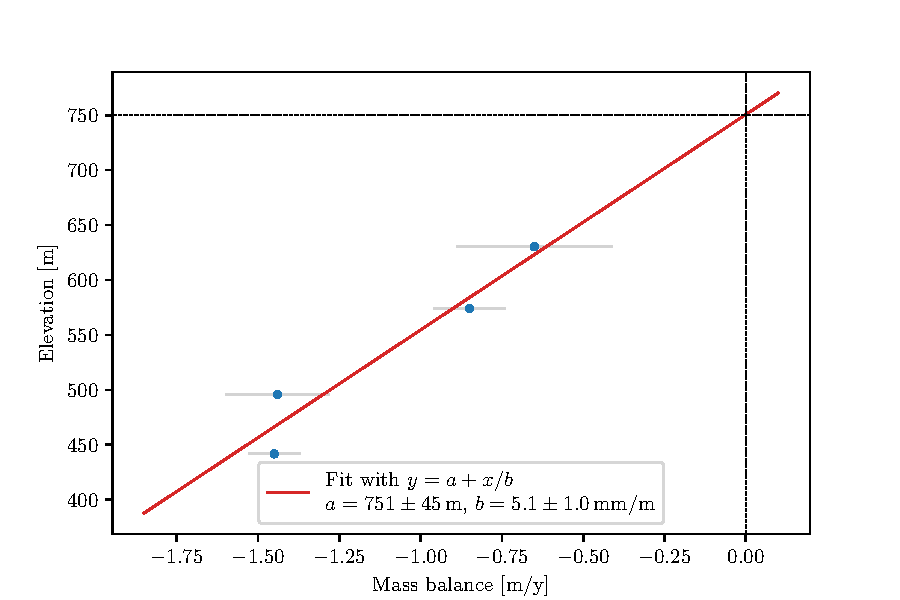
\includegraphics[width=\textwidth]{./figs/Elevation_Blekumbreen_mbg.pdf}
    \caption{Mass balances of the stakes on Blekumbreen as a function of stake elevation and linear fit of the points to obtain
    the equilibrium line elevation $a$ and the mass balance gradient $b$.}
    \label{GPS:fig:elev_ble_mbg}
\end{figure}


\begin{figure}[htb]
    \centering
    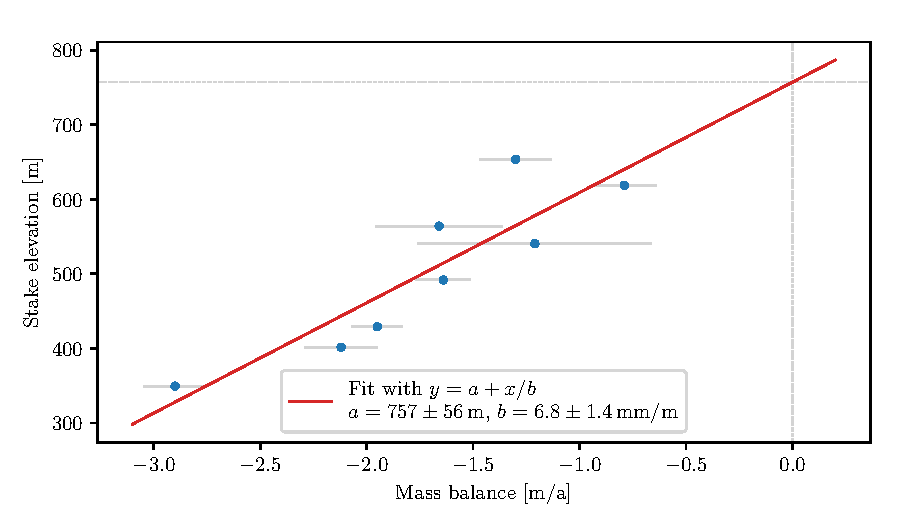
\includegraphics[width=\textwidth]{./figs/Elevation_Tellbreen_mbg.pdf}
    \caption{Mass balances of the stakes on Tellbreen as a function of stake elevation and linear fit of the points to obtain
    the equilibrium line elevation $a$ and the mass balance gradient $b$.}
    \label{GPS:fig:elev_tel_mbg}
\end{figure}

\subsection{Theoretical surface velocity}
% Different tables for different values of B(T = 0,-5,-10,-15), \alpha = 5,6,7 and H (from the ice-radar scans) = 1 (minimal value — minimum was at 3), 33.4 (average value), 82,3 (maximum)
Based on the shallow ice approximation it is possible to calculate a theoretical surface velocity for the glaciers we did our measurements on.
To make the calculation (Eq.~\ref{GPS:eq:sia}) the variables slope angle, ice velocity and ice thickness have to be chosen. 
The ice density is assumed as 917 kg/m$^3$ and the gravitational acceleration as 9.81  m/s$^2$.
The values for the ice viscosity are displayed in Table \ref{GPS:tab:iceviscosities}.
It is not possible to determine the exact ice temperature.
Because of this, the calculation is done for different viscosities at specific ice temperatures $T$.

\begin{table}[htb]
\centering
\begin{tabular}{lcccc}
\toprule
Temperature [$^\circ$C] & 0 & -5 & -10 & -15 \\
\midrule
Ice viscosity $\left[ P / \text{a}^{-3} \right]$ & $5,52 \cdot 10^7$ & $8,63 \cdot 10^7$ & $1.28 \cdot 10^8$ & $1.52 \cdot 10^8$\\
\bottomrule
\end{tabular}
\caption{Ice viscosities for different ice temperatures $T = \{0,-5,-10,-15\}$}
\label{GPS:tab:iceviscosities}
\end{table}

The theoretical velocity is mainly influenced by the ice thickness (see Tables \ref{GPS:tab:theorytable5}, \ref{GPS:tab:theorytable6} and \ref{GPS:tab:theorytable7} ).
For the mean thickness the theoretical surface velocity of ice has the order of magnitude of centimeters. 
The small velocity values correspond with the measured velocities (see Table~ \ref{GPS:tab:vel_tab}). 

\begin{table}[htb]
    \centering
    	\caption{Theoretical surface velocity $u_\circledS\,\left[m / \text{a} \right]$, $\alpha = 5$}
	\begin{tabular}{lccc}
	\toprule
	$\alpha=5$ & $H_{min} = 1$ & $H_{avg}=33.4$ & $H_{max} = 82.3$\\
	\midrule
	B($T=0$ C) & $4.51 \cdot 10^{-8}$ & $5.61 \cdot 10^{-2}$ & $2.07$ \\
	B($T=-5$ C) & $1.18 \cdot 10^{-8}$ & $1.47 \cdot 10^{-2}$ & $5.43 \cdot 10^{-1}$ \\
	B($T=-10$ C) & $3.63 \cdot 10^{-9}$ & $4.51 \cdot 10^{-3}$ & $1.17 \cdot 10^{-1}$ \\

	B($T=-15$ C) & $2.17 \cdot 10^{-9}$ & $2.71 \cdot 10^{-3}$ & $9.98 \cdot 10^{-2}$\\
	\bottomrule	
	\end{tabular}
	\label{GPS:tab:theorytable5}
	
	\caption{Theoretical surface velocity $u_\circledS\,\left[m / \text{a} \right]$, $\alpha = 6$}
	\begin{tabular}{lccc}
	\toprule
	$\alpha=6$  & $H_{min} = 1$ & $H_{avg}=33.4$ & $H_{max} = 82.3$ \\
	\midrule
	B($T=0$ C) & $7.78 \cdot 10^{-8}$ & $9.68 \cdot 10^{-2}$ & $3.57$ \\

	B($T=-5$ C) & $2.04 \cdot 10^{-8}$ & $2.54 \cdot 10^{-2}$ & $9.37 \cdot 10^{-1}$ \\
	B($T=-10$ C) & $6.26 \cdot 10^{-9}$ & $7.79 \cdot 10^{-3}$ & $2.87 \cdot 10^{-1}$ \\
	B($T=-15$ C) & $3.75 \cdot 10^{-9}$ & $4.67 \cdot 10^{-3}$ & $1.72 \cdot 10^{-1}$\\
	\bottomrule	
	\end{tabular}
	\label{GPS:tab:theorytable6}
    
    \caption{Theoretical surface velocity $u_\circledS\,\left[m / \text{a} \right]$, $\alpha = 7$}
	\begin{tabular}{lccc}
	\toprule
	$\alpha=7$  & $H_{min} = 1$ & $H_{avg}=33.4$ & $H_{max} = 82.3$ \\
	\midrule
	B($T=0$ C) & $1.23 \cdot 10^{-7}$ & $1.53 \cdot 10^{-1}$ & $5.66$ \\
	B($T=-5$ C) & $3.24 \cdot 10^{-8}$ & $4.03 \cdot 10^{-2}$ & $1.49$ \\
	B($T=-10$ C) & $9.92 \cdot 10^{-9}$ & $1.23 \cdot 10^{-2}$ & $4.55 \cdot 10^{-1}$ \\
	B($T=-15$ C) & $5.95 \cdot 10^{-9}$ & $7.40 \cdot 10^{-3}$ & $2.73 \cdot 10^{-1}$\\
	\bottomrule	
	\end{tabular}
	\label{GPS:tab:theorytable7}
\end{table}

The theoretical calculation can be applied on the different stake locations.
The surface velocities for the ice temperatures of -5$^\circ$C and -10$^\circ$C are comparable results to the measurement values (see Table~\ref{GPS:tab:stakesvelocities}).
Also the calculated mass balances confirm with the negative values of both glaciers which are completely in their ablation zones (see Subsection~\ref{GPS:subsec:maba}). 

\begin{table}[htb]
    \centering
    
    \footnotesize
    \caption{Theoretical surface velocity at all the stakes. "no data" translates into an absence of data for the Ice Thickness (I. T.)}
	\begin{tabular}{lcccccc}
	\toprule
Stake & Northing [m] & Easting [m] & I. T. [m] & $u_\circledS^{T=-5}\,[m / \text{a}]$ & $u_\circledS^{T=-10}$ [$m / \text{a}$] & Mass bal. [$m / \text{a}$]\\
\midrule
BL2-2018 & 8686150 & 523051 & 66.48 & 0.40 & 0.12 & -1.1475\\
BL3-2018 & 8686091 & 523545 & 53.46 & 0.17 & 0.05 & -0.9095\\
BL4-2018 & 8686099 & 524181 & 34.96 & 0.03 & 0.01 & -0.6885\\
BL5-2017 & 8686131 & 524644 & 75.92 & 0.68 & 0.21 & -0.119\\
T1-2018 & 8687107 & 528388 & no data & - & - & -2.108\\
T2-2018 & 8687320 & 527951 & no data & - & - & -1.42375\\
T3-2017 & 8687273 & 527598 & no data & - & - & -1.1985\\
T4-2018 & 8687138 & 527125 & 47.09 & 0.10 & 0.03 & -0.731\\
T5-2018 & 8686938 & 526691 & 61.97 & 0.30 & 0.09 & -0.646\\
T6-2018 & 8686675 & 526247 & 69.80 & 0.48 & 0.15 & -0.323\\
T7-2017 & 8686579 & 525858 & 55.68 & 0.20 & 0.06 & -0.221\\
T8-2017 & 8686472 & 525524 & 27.28 & 0.01 & 0.00 & -0.5525\\
\bottomrule
	\end{tabular}
	\label{GPS:tab:stakesvelocities}
\end{table}
\FloatBarrier

\section{Discussion} \label{GPS:sec:Discussion}
\subsection{Data processing}


\subsection{Horizontal velocity}


\subsection{Vertical velocity}


equlilbrium line not on the glacier

equilibrium lines and mass balances are the same within their uncertainties


comparison with mass balance group data

our data could be more precise than measurements of single years, because statistical fluctuations of single years have less influence



higher ablation at T6 and T8: Due to local environment (mountains, inclination, wind, sun...)






\section{Conclusion}
The new open source post processing method provides similar results for the stake positions.
Therewith the licensed TBC sofware can be replaced by the open source method.
Based on the results of the measured and theoretically calculated ice velocities we can confirm the low velocities measured the last years.
Due to a lot uncertainties in the measurement setup the uncertaint can only hardly reduced.
The uncertainties with 0.40 m for northing and 0.19 m for easting are the upper limit for the velocities. 
This leads to an high error in the velocity so the horizontal velocity not measurable.
But because of a faster movement in the vertical direction it is possible to calculate even with an uncertainty of 0.89 m, a vertical velocity.
Thus we are able to calulate a mass balance for both glacier, which shows us that the whole area of the glacier is in the ablation zone.
The theoretical surface velocity out of the shallow ice approximation validate the small values for the horizontal velocity.
Prospective, the measurement setup should be improved. 
Since, we tried the best of documentation and correction of the measurement data it is even not possible to reduce the uncertainties of the positioning and velocity significantly. 
The suggestion for the improvement is to drill the stakes defenetly straight to avoid a too high inclination.
Also the rover should be placed every time on top of the stake.
If the stake is to high melted out, it should be cut. 
This has to be documented very well too- 
Open source software can be used instead of TBC



uncertainties of tab 1.1 is upper limit for velocity

Horizontal velocity not measurable, better vertical.



Improvements...

-> put stakes straight
-> put rover in stake, cut stake
-> measure more stakes two times




%-------------- References ---------------------
% DON'T CHANGE ANYTHING IN THE FOLLOWING LINES!!!
%\section*{References}
%\begin{btSect}{studentxx/literature}
%\btPrintCited
%\end{btSect}


%% This is the ReportPart.tex file. Here comes all your text, tables, figures. When you want to compile the document, compile Compile.tex, and NOT ReportPart.tex.
% At first fill in the first three commands before the abstract: Your name as the chapters author, the chapter title and the lable of the whole chapter.

%%%%%%%%%%%%%%%%%%%%%%%%%%%%%%%%%%%%%%%%%%%%%%%%%%%%%%%%%%%%%%%%%%%%%%%%%%%%%%%%%%%%%%%%%%5

\renewcommand{\chapterauthor}{Write your name here}
\chapter{Chapter title}
\label{studentxx:report}

%--------------- Abstract ----------------------
\begin{abstract}

That's gonna be the abstract...

\end{abstract}

%-------------- Introduction -------------------

\section{Introduction}

And here's the Introduction...


%-------------- References ---------------------
% DON'T CHANGE ANYTHING IN THE FOLLOWING LINES!!!
%\section*{References}
%\begin{btSect}{studentxx/literature}
%\btPrintCited
%\end{btSect}


%% This is the ReportPart.tex file. Here comes all your text, tables, figures. When you want to compile the document, compile Compile.tex, and NOT ReportPart.tex.
% At first fill in the first three commands before the abstract: Your name as the chapters author, the chapter title and the lable of the whole chapter.

%%%%%%%%%%%%%%%%%%%%%%%%%%%%%%%%%%%%%%%%%%%%%%%%%%%%%%%%%%%%%%%%%%%%%%%%%%%%%%%%%%%%%%%%%%5

\renewcommand{\chapterauthor}{Write your name here}
\chapter{Chapter title}
\label{studentxx:report}

%--------------- Abstract ----------------------
\begin{abstract}

That's gonna be the abstract...

\end{abstract}

%-------------- Introduction -------------------

\section{Introduction}

And here's the Introduction...


%-------------- References ---------------------
% DON'T CHANGE ANYTHING IN THE FOLLOWING LINES!!!
%\section*{References}
%\begin{btSect}{studentxx/literature}
%\btPrintCited
%\end{btSect}


%   .
%   .
%   .

%%%%%%%%%%%%%%%%%%% APPENDIX %%%%%%%%%%%%%%%
\begin{appendices}
   % That is the appendix. Just add stuff. that you do not want to include in the main report but still want to show. here.
% Name the label to for example "student03:appendix" if you are student 03 so that you can refer to your appendix in your ReportPart by using "\ref{student03:appendix}"
% No referencing in appendix implemented yet.

%%%%%%%%%%%%%%%%%%%%%  John Doe  %%%%%%%%%%%%%%%%%%%%%

\chapter{Appendix YOUR-PROJECT-NAME}
\label{studentxx:appendix}


Raw data from fieldbook.
% raw position data from the Trimble Controller
\begin{table}[h]
\caption{Raw position data in Northing, Easting and Elevation from the Trimble Controller.}
\centering
\begin{tabular}{lccc}
\toprule
        Name & Northing [m] & Easting [m] & Elevation [m] \\
\midrule
    BL2-2016 &   8686150.91 &   523049.58 &        441.45 \\
    BL2-2018 &   8686149.18 &   523052.26 &         439.6 \\
    BL3-2016 &   8686090.70 &   523545.65 &        486.42 \\
    BL3-2018 &   8686090.05 &   523546.95 &        485.58 \\
    BL4-2018 &   8686100.72 &   524179.05 &        569.47 \\
  BL4-i-2016 &   8686098.16 &   524180.50 &        577.73 \\
 BL4-ii-2016 &   8686099.46 &   524180.49 &        575.12 \\
  BL5-i-2017 &   8686132.09 &   524644.27 &         631.4 \\
 BL5-ii-2017 &   8686128.59 &   524645.35 &        624.69 \\
     T1-2018 &   8687106.45 &   528388.09 &        343.82 \\
   T1-i-2017 &   8687106.51 &   528389.87 &         342.4 \\
  T1-ii-2017 &   8687104.86 &   528388.57 &         340.5 \\
     T2-2016 &   8687322.63 &   527951.49 &        400.25 \\
     T2-2018 &   8687318.62 &   527951.78 &        391.96 \\
   T2-i-2017 &   8687321.16 &   527951.98 &        393.06 \\
  T2-ii-2017 &   8687321.10 &   527952.02 &         396.3 \\
     T3-2017 &   8687273.68 &   527599.16 &        428.93 \\
     T4-2016 &   8687138.55 &   527125.09 &         490.1 \\
     T4-2018 &   8687138.56 &   527125.09 &         490.1 \\
     T5-2016 &   8686940.26 &   526691.93 &        538.15 \\
     T5-2018 &   8686939.86 &   526689.56 &        548.25 \\
     T6-2016 &   8686676.52 &   526249.39 &        568.05 \\
     T6-2018 &   8686673.79 &   526246.38 &        559.77 \\
     T7-2015 &   8686579.41 &   525858.64 &        612.84 \\
     T7-2017 &   8686378.63 &   525858.64 &        615.19 \\
     T8-2017 &   8686471.63 &   525524.23 &        650.45 \\
\bottomrule
\end{tabular}

\label{GPS:tab:fb_pos_tab}
\end{table}

% raw data from the measurements in the field
\begin{table}[h]
\caption{Raw data collected in the field used for the stake correction.}
\centering
\begin{tabular}{lllllll}
\toprule
        Name &        Date & Antenna height [m] & Snow depth [m] & Inclination [deg] & Direction of Incl. [deg] & Distance Rover-Stake [m] \\
\midrule
    BL2-2016 &  15.03.2018 &               2.18 &            1.1 &                 3 &                      225 &                     0.18 \\
    BL2-2018 &  15.03.2018 &                0.6 &              0 &                 2 &                      270 &                        0 \\
    BL3-2016 &  15.03.2018 &                2.2 &           1.07 &                12 &                      270 &                      0.1 \\
    BL3-2018 &  15.03.2018 &                0.6 &              0 &                 0 &                        0 &                        0 \\
    BL4-2018 &  15.03.2018 &               0.92 &              0 &                 0 &                        0 &                        0 \\
  BL4-i-2016 &  15.03.2018 &               2.08 &           0.93 &                10 &                      270 &                     0.11 \\
 BL4-ii-2016 &  16.03.2018 &               1.25 &           1.25 &                10 &                      270 &                      0.2 \\
  BL5-i-2017 &  15.03.2018 &               1.32 &            1.1 &                 0 &                        0 &                        0 \\
 BL5-ii-2017 &    16.03.18 &               0.48 &            1.3 &                 0 &                        0 &                        0 \\
     T1-2018 &  13.03.2018 &               0.66 &              0 &                 0 &                        0 &                        0 \\
   T1-i-2017 &  11.03.2018 &                2.2 &            0.8 &                 9 &                      180 &                     0.15 \\
  T1-ii-2017 &  13.03.2018 &               2.15 &            0.8 &                10 &                      180 &                     0.17 \\
     T2-2016 &  15.03.2018 &               1.34 &           0.97 &                 0 &                        0 &                      0.1 \\
     T2-2018 &  13.03.2018 &               0.66 &              0 &                 5 &                      225 &                        0 \\
   T2-i-2017 &  11.03.2018 &               2.23 &              1 &                10 &                       90 &                      0.1 \\
  T2-ii-2017 &  13.03.2018 &                1.4 &              1 &                 5 &                      135 &                      0.1 \\
     T3-2017 &  11.03.2018 &               1.87 &           1.05 &                 0 &                        0 &                      0.1 \\
     T4-2016 &  11.03.2018 &               2.42 &            1.2 &                 5 &                        0 &                      0.1 \\
     T4-2018 &  13.03.2018 &               0.63 &              0 &                 0 &                        0 &                        0 \\
     T5-2016 &  11.03.2018 &               2.44 &           1.22 &                 8 &                        0 &                      0.1 \\
     T5-2018 &  15.03.2018 &               0.45 &              0 &                 0 &                        0 &                        0 \\
     T6-2016 &  11.03.2018 &                2.3 &           1.35 &                 4 &                      180 &                     0.15 \\
     T6-2018 &  15.03.2018 &               1.95 &            1.4 &                 0 &                        0 &                        0 \\
     T7-2015 &  13.03.2018 &               1.84 &            1.2 &                10 &                       45 &                      0.1 \\
     T7-2017 &  13.03.2018 &               0.98 &           1.21 &                 0 &                        0 &                        0 \\
     T8-2017 &  13.03.2018 &               2.09 &            0.7 &                 5 &                      180 &                      0.1 \\
\bottomrule
\end{tabular}

\label{GPS:tab:fb_other_tab}
\end{table}

% final positions post processed with the Trimble Business Center.
\begin{table}[h]
\caption{Final positions in Northing, Easting and Elevation with the TBC post processing and the stake correction.}
\centering 
\begin{tabular}{lrrr}
\toprule
        Name &  Northing [m] &  Easting [m] &  Elevation [m] \\
\midrule
    BL2-2016 &    8686150.51 &    523049.54 &         436.86 \\
    BL2-2018 &    8686149.27 &    523051.55 &         437.76 \\
    BL3-2016 &    8686092.71 &    523543.82 &         491.07 \\
    BL3-2018 &    8686091.13 &    523545.37 &         491.15 \\
    BL4-2018 &    8686098.89 &    524181.02 &         571.86 \\
  BL4-i-2016 &    8686099.66 &    524179.06 &         571.55 \\
 BL4-ii-2016 &    8686099.30 &    524179.33 &         571.36 \\
  BL5-i-2017 &    8686129.64 &    524644.30 &         628.64 \\
 BL5-ii-2017 &    8686129.44 &    524644.29 &         628.61 \\
     T1-2018 &    8687106.61 &    528388.32 &         341.43 \\
   T1-i-2017 &    8687105.34 &    528388.87 &         341.25 \\
  T1-ii-2017 &    8687105.06 &    528388.51 &         341.30 \\
     T2-2016 &    8687320.86 &    527951.55 &         395.12 \\
     T2-2018 &    8687319.67 &    527950.59 &         395.13 \\
   T2-i-2017 &    8687320.99 &    527951.91 &         395.17 \\
  T2-ii-2017 &    8687320.68 &    527951.29 &         395.25 \\
     T3-2017 &    8687273.10 &    527598.30 &         422.57 \\
     T4-2016 &    8687141.52 &    527123.96 &         486.78 \\
     T4-2018 &    8687137.40 &    527124.77 &         487.25 \\
     T5-2016 &    8686935.92 &    526692.26 &         534.57 \\
     T5-2018 &    8686937.70 &    526690.76 &         535.26 \\
     T6-2016 &    8686673.29 &    526248.19 &         561.86 \\
     T6-2018 &    8686674.33 &    526246.57 &         560.49 \\
     T7-2015 &    8686581.42 &    525859.20 &         615.80 \\
     T7-2017 &    8686579.33 &    525858.40 &         615.81 \\
     T8-2017 &    8686470.03 &    525522.18 &         649.70 \\
\bottomrule
\end{tabular}

\label{GPS:tab:tbc_tab}
\end{table}
%   \include{./appendix/instrument2}
    %   .
    %   .
    %   .
\end{appendices}

\end{document}
